\listfiles
\documentclass[review]{elsarticle}

\usepackage{lineno,hyperref}
\modulolinenumbers[5]

\journal{Journal of \LaTeX\ Templates}

%%%%%%%%%%%%%%%%%%%%%%%
%% Elsevier bibliography styles
%%%%%%%%%%%%%%%%%%%%%%%
%% To change the style, put a % in front of the second line of the current style and
%% remove the % from the second line of the style you would like to use.
%%%%%%%%%%%%%%%%%%%%%%%

% Numbered
% \bibliographystyle{model1-num-names}

%% Numbered without titles
% \bibliographystyle{model1a-num-names}

%% Harvard
% \bibliographystyle{model2-names}\biboptions{authoryear}

%% Vancouver numbered
% \usepackage{numcompress}\bibliographystyle{model3-num-names}

%% Vancouver name/year
% \usepackage{numcompress}\bibliographystyle{model4-names}\biboptions{authoryear}

%% APA style
% \bibliographystyle{model5-names}\biboptions{authoryear}

%% AMA style
% \usepackage{numcompress}\bibliographystyle{model6-num-names}

\usepackage{graphicx}
\graphicspath{ {figures/} }
%% `Elsevier LaTeX' style, distributed in TeX Live 2019
\bibliographystyle{elsarticle-num}
% \usepackage{numcompress}\bibliographystyle{elsarticle-num-names}
% \bibliographystyle{elsarticle-harv}\biboptions{authoryear}
%%%%%%%%%%%%%%%%%%%%%%%

\begin{document}

\begin{frontmatter}

\title{Comparative Performance Evaluation of Hadoop on PaaS Proposals by Leveraging HiBench}
\tnotetext[mytitlenote]{Fully documented templates are available in the elsarticle package on \href{http://www.ctan.org/tex-archive/macros/latex/contrib/elsarticle}{CTAN}.}

%% Group authors per affiliation:
\author{Elsevier\fnref{myfootnote}}
\address{Radarweg 29, Amsterdam}
\fntext[myfootnote]{Since 1880.}

%% or include affiliations in footnotes:
\author[mymainaddress,mysecondaryaddress]{Elsevier Inc}
\ead[url]{www.elsevier.com}

\author[mysecondaryaddress]{Global Customer Service\corref{mycorrespondingauthor}}
\cortext[mycorrespondingauthor]{Corresponding author}
\ead{support@elsevier.com}

\address[mymainaddress]{1600 John F Kennedy Boulevard, Philadelphia}
\address[mysecondaryaddress]{360 Park Avenue South, New York}

\begin{abstract}
As rapid as in only the last two decades the advent of Big Data emerged in any data-driven domain and scaled up the extent as well as the depth of data and its handling. In an ongoing maturing process, new approaches leaning on enhanced distributed storage and computing paradigms are invented helping overcome management and running analytics challenges. In this context Hadoop is a success story embraced by a wide scale of beneficiants both from industry and academia since its first release in 2005. The commercialization of Cloud Computing started a grand migration movement towards cloud, applying also for Hadoop transferring its presence from on-premises to virtual machines stored and tamed in large data center facilities by global Cloud Service Providers. The CSPs' response to result-focused analytics needs of business purposes emerged a new service called managed systems where the hard workload of multi node cluster implementation is overtaken by the contractor in providing a pre-configured Hadoop package simplifying the installation process to a matter of property selection thus eliminating technical know-how requirements on such an implementation. Converting the concept of cloud based Hadoop from IaaS to PaaS apparently reduced costs commercially presented as pay-as-you-go or pay-per-use. There is a payoff, though, managed Hadoop systems do present a black-box behavior to the end user who cannot be clear on the inner dynamics, hence the benefits by leveraging them. In this study we selected three global providers (GCP, Azure, and Alibaba Cloud), activated their Hadoop PaaS services (Dataproc, HDInsight, and e-MapReduce, respectively) within same geographical region and by promise apparently same computing specifications, and executed several Hadoop workloads of the HiBench Benchmark Suite. The results yield that selecting apparently same computation specs among CSPs' services does not necessarily guarantee equal or close performance outputs among them. Our assumption is that pre-configuration work of managed systems done by the contractors play a weighing role on their performance.
\end{abstract}

\begin{keyword}
%%\texttt{elsarticle.cls}\sep \LaTeX\sep Elsevier \sep template
\texttt{elsarticle.cls}\sep Benchmark Hadoop PaaS\sep HiBench\sep Performance evaluation

\MSC[2010] 00-01\sep  99-00
\end{keyword}

\end{frontmatter}

\linenumbers

%%\section{The Elsevier article class}
\section{Introduction}

Big Data has become an inevitable aspect for enterprises and academia of the information era to deal with. As the global internet access rate covers a weighing majority of the global human population, mobile technology devices become democratized, sensors and IoT devices the more occupy daily life, ongoing scientific researches produce vast amounts of data outputs the Big Data phenomenon gathered itself by means of overwhelming size with Volume, ever accelerating growth rate with Velocity, and splitting into diverse structures with Variety, new approaches were forced to mature in order to ease the maintenance of Big Data and enable extracting valuable insights from it leveraging complex statistical formulae. Distributed frameworks for storage and computation sparked up first by search engines were inherited and furtherly developed by the open source community yielding what is known as Hadoop and its ecosystem today. Considering the complexity of dealing with big data Hadoop represents a modern analytics framework decreasing management efforts and duration of analytics operations to an acceptable level by means of affordable commodity computers.

In parallel, the commercialization of Cloud Computing in the early 2000's delivered utilization of storage and computing resources to the end users saving them high investments on hardware technology that is soon going to be obsolete and is expensive to maintain. As the migration to the cloud is an ongoing process, Hadoop also slips out from its residence on on-prem infrastructure to the cloud by being implemented on virtual machine instances provided as IaaS platforms by many providers. The Cloud Service Providers embraced the need of eliminating Hadoop's complex implementation process on multi-node VMs by providing managed Hadoop systems commercially packaged as PaaS, which are pre-installed and pre-configured Hadoop clusters allowing the installation of tens to hundreds of nodes in a matter of minutes by simply determining some settings like hardware specs and node numbers prior the installation. The Managed Hadoop system is both a blessing and a curse, by leaving the hard implementation part which is not necessarily related with the main analysis objective to a contractor the end user saves time and efforts including a payoff, though: By definition, managed systems are prepackaged solutions provided in black-box nature. CSP apply behind-the-scenes tweaks in terms of reaching better performance results on selected approaches like memory intensive or compute intensive applications.

In this study we put three CSP providers' managed Hadoop services in focus in terms of performance evaluation comparison: GCP Dataproc, Azure HDInsight, and Alibaba Cloud e-MapReduce, each recognized in Gartner's 2020 report in leading or niche section. Bound by availability of their offered hardware and software options we selected by providers' promise apparently same or close settings. Without any tweak operation with their settings for any performance optimization on the respective managed systems after installation we immediately executed several workloads from HiBench's micro, sql, ml, and websearch categories. For a more clear understanding of the benchmark outputs, during the benchmark execution we collected system utilization records on each worker node of the cluster. The results yield that Hadoop PaaS offerings by vendor's promise side perform and system utilizations may highly vary among CSPs.

\paragraph{Installation} If the document class \emph{elsarticle} is not available on your computer, you can download and install the system package \emph{texlive-publishers} (Linux) or install the \LaTeX\ package \emph{elsarticle} using the package manager of your \TeX\ installation, which is typically \TeX\ Live or Mik\TeX.

\paragraph{Usage} Once the package is properly installed, you can use the document class \emph{elsarticle} to create a manuscript. Please make sure that your manuscript follows the guidelines in the Guide for Authors of the relevant journal. It is not necessary to typeset your manuscript in exactly the same way as an article, unless you are submitting to a camera-ready copy (CRC) journal.

\paragraph{Functionality} The Elsevier article class is based on the standard article class and supports almost all of the functionality of that class. In addition, it features commands and options to format the
\begin{itemize}
\item document style
\item baselineskip
\item front matter
\item keywords and MSC codes
\item theorems, definitions and proofs
\item lables of enumerations
\item citation style and labeling.
\end{itemize}


\section{Related Work}
HiBench is a tool to measure a specific system’s performing behaviour during execution. The conceptualization of conducting a benchmark may arise from different soils. Based on the conductor’s motivation; a benchmark’s use case could be an inner evaluation of a system’s performance before and after some configuration tweaks are set, comparison of rival / complementary systems, or putting CSP’s cloud infrastructure services on scale. Following literature has been searched with finding different use cases of HiBench benchmarking suite in mind. 

Poggi et al. [52] Characterizing BigBench…

Poggi et al. the state of SQL on Hadoop [53]…

Samadi et al. conduct an experimental comparison between Spark and Hadoop installed on virtual machines on Amazon EC2 by leveraging nine among the provided HiBench workloads. Accuracy reasons led the conductors run the workloads three times concluding input data scales of 1, 3, and 5 GB respectively. Based on the outputs comprising duration, throughput, speed up, and CPU/memory consumption, the conclusion draws Spark consuming less CPU and performing better on all workload results over Hadoop. 

Ahn et al. [54] put Spark on YARN’s performance on test with HiBench in terms of handling a deluge of data generated by IoT devices. The experiment is run on a cluster with one master and 3 worker nodes each node possessing Intel® Xeon® processor with 20 cores and 128GB main memory meaning 60 cores and 384GB memory in total. HiBench’s workloads Micro (comprising Sort, TeraSort, and Wordcount), SQL (comprising Aggregation, Join, and Scan), and Machine Learning (comprising Bayes, Logistic Regression, Gradient Boosting Tree, Random Forest, and Linear Regression) are leveraged by a chosen data scale of 30 GB. Spark occupies memory during the whole job execution which in result reduces IOs’ negative impact on processor performance. For optimizing resource usage the conductors modified YARN’s minimum memory allocation and Spark executor settings so that the Spark executors’ overall loads remain below total system memory. Alongside with HiBench’s duration and throughput report, CPU / memory utilization and disk throughput are profiled as well. Finding of this paper points out that Spark guarantees performance when provided with enough memory.

Han et al. [55] study the impact of memory size on big data processing by means of Hadoop and Spark performance comparison leveraging HiBench’s k-Means workload as the only benchmark. For each of the specified memory sizes of 4, 8, and 12 GB, iterating through a data scale of 1 to 8 GB, with 1GB increment inbetween, k-Means benchmark for Hadoop and Spark is executed. The results depict Spark’s overperforming Hadoop unless the total input data size is smaller than 33.5\% of the total memory size assigned to worker nodes. After reaching that ratio Spark suffers with insufficient memory resources and is led to interoperate with HDFS causing a sharp decrease in its performance and brings Hadoop in throughput and duration performance to the front. The conductors make a second experiment to find out if Spark’s performance can be improved by tweaking the allocation setting for storage memory and shuffle memory while remaining within the specified memory limitations of 4, 8 and 12 GB. Executing HiBench’s k-means benchmark outputs a report interpreted by the conducters as Spark show a 5-10\%, and 15\% maximum improvement in processing time.

Ivanov et al. [56] compare the performances of two enterprise grade applications, DataStax Enterprise (DSE), a production level implementation of Apache Cassandra with extended features like in memory computing and advanced security to name but two, and Cloudera’s Distribution of Hadoop (CDH) comprising core Hadoop elements HDFS and YARN integrated with elements belonging to the Hadoop ecosystem. DSE’s HDFS compatible file system CSF lets Hadoop applications run without any modification. The conductors installed the latest stable releases of both softwares on equal CPU, memory and network infrastructure configuration. For both installations, default system parameters have been left with their defaults. HiBench’s three chosen workloads (CPU-bound wordcount, IO-bound dfsioe, and mixed HiveBench) are executed three times, the average values have been taken for representativeness. Several conclusions of their study proclaim linearly scaling of both systems by the increase of data size, while CDH outperforms DSE in read intensive workloads, DSE performs better in write intensive workloads. Leveraging HiBench is where this study differs in approach related to other studies using YCSB benchmark suite. HiBench’s results confirm the latter’s output as well.




\section{Method}

\section{Results}
HiBench's Hadoop related benchmarks in groups micro (Sort, Terasort, Dfsioe, and Wordcount), sql (Scan, Join, and Aggregation), ml (Bayes and Kmeans), and websearch (Pagerank) have been executed on all three CSPs managed Hadoop services. During benchmark runtime resource utilization on worker nodes have been captured. The resulting multiplots are suggested to be read as follows: Top-left, top-right, and bottom-left plots represent CPU (user\%), Memory, and IO utilization on each worker node of the respective cluster over time. CPU utilization lines are given in blue tones, Memory utilization lines are given in fuchsia tones, IO-read and IO-write tps' are represented with orange tones and green tones, respectively. Even though the coloring convention might sound confusing, it gives a clear overview in terms of resource utilization of the total benchmark process over time. The left hand side x-axis measures CPU/Memory usage in percent, the right hand side x-axis measures IO-read or IO-write transfers in byte per second. The bottom-right plot represents the comparative benchmark performance outputs of the respective CSP. Duration measure in seconds is expected to perceived as "lower is better" while Throughput which is the amount of processed data per second in bytes is expected to perceived as "higher is better".

USE CASE 1: 

\paragraph{Sort - Huge} Lorem ipsum

\paragraph{Sort - Gigantic} Lorem ipsum

\paragraph{Terasort - Huge} Lorem ipsum

\paragraph{Terasort - Gigantic} Lorem ipsum

\paragraph{Dfsioe-read - Huge} Lorem ipsum

\paragraph{Dfsioe-read - Gigantic} Lorem ipsum

\paragraph{Dfsioe-write - Huge} Lorem ipsum

\paragraph{Dfsioe-write - Gigantic} Lorem ipsum

\paragraph{Wordcount - Huge} Lorem ipsum

\paragraph{Wordcount - Gigantic} Lorem ipsum

\paragraph{Scan - Huge} Lorem ipsum

\paragraph{Scan - Gigantic} Lorem ipsum

\paragraph{Join - Huge} Lorem ipsum

\paragraph{Join - Gigantic} Lorem ipsum

\paragraph{Aggregation - Huge} Lorem ipsum

\paragraph{Aggregation - Gigantic} Lorem ipsum

\paragraph{Bayes - Huge} Lorem ipsum

\paragraph{Bayes - Gigantic} Lorem ipsum

\paragraph{Kmeans - Huge} Lorem ipsum

\paragraph{Kmeans - Gigantic} Lorem ipsum

\paragraph{Pagerank - Huge} Lorem ipsum

\paragraph{Pagerank - Gigantic} Lorem ipsum

\begin{figure}[b]
	\caption{UC1 - Sort (Huge; 3.2 GB)}
	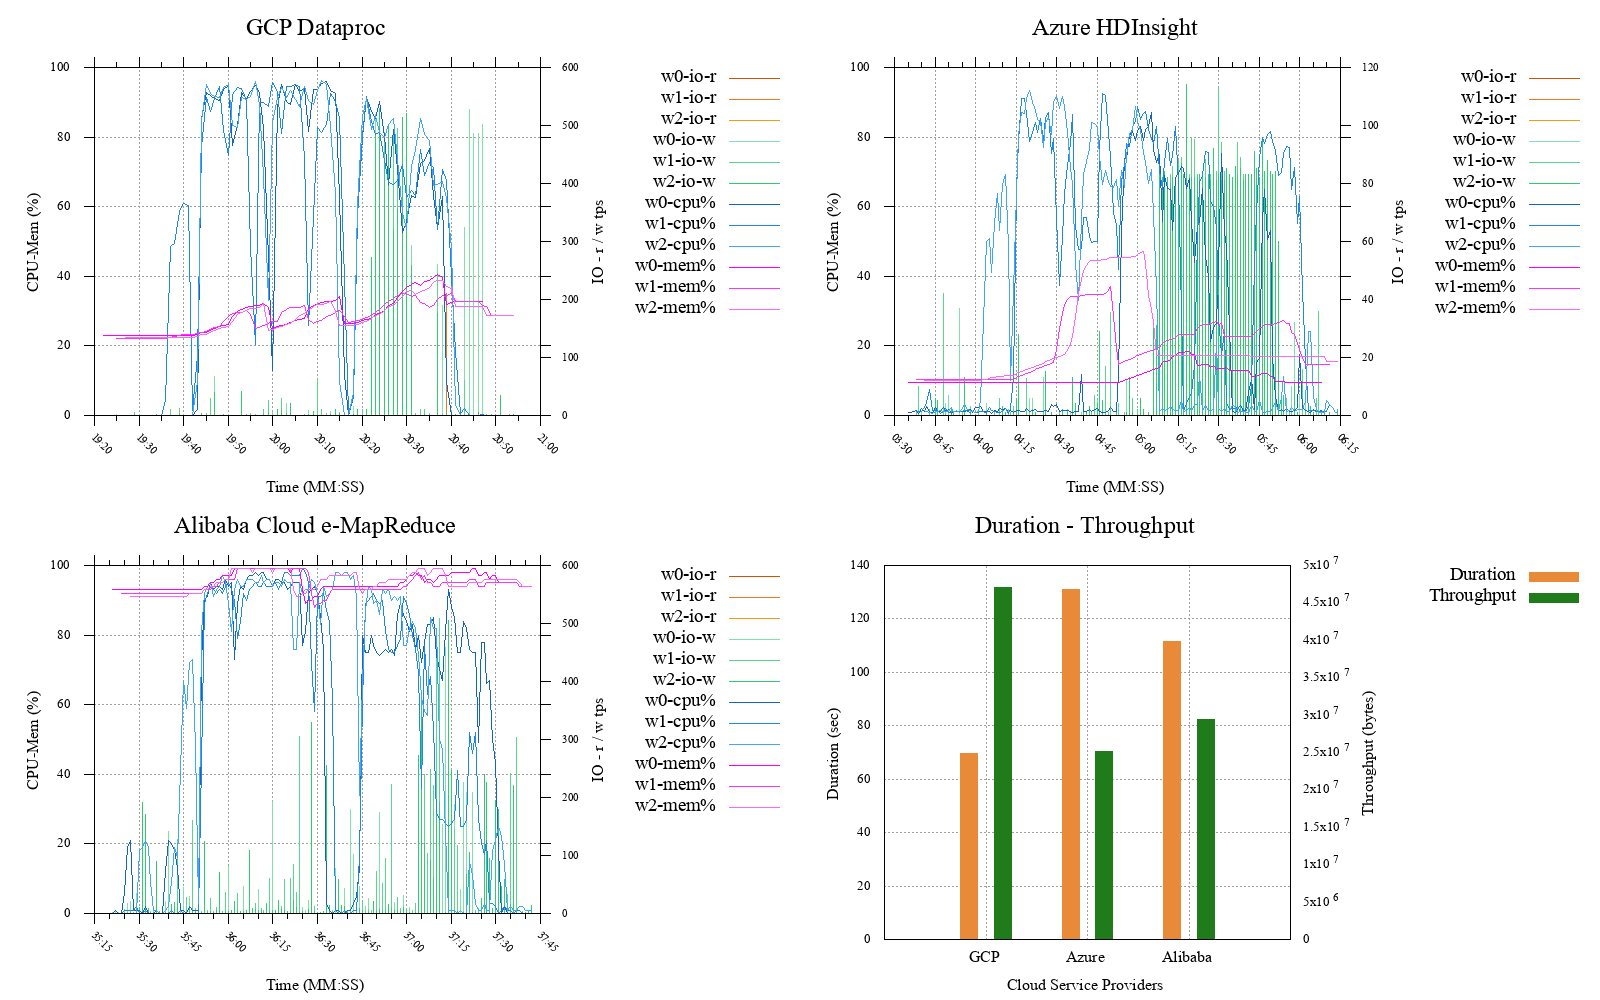
\includegraphics[width=\textwidth]{uc1-srt-h-cmidt}
	\centering
\end{figure}

\begin{figure}[b]
	\caption{UC1 - Sort (Gigantic; 32 GB)}
	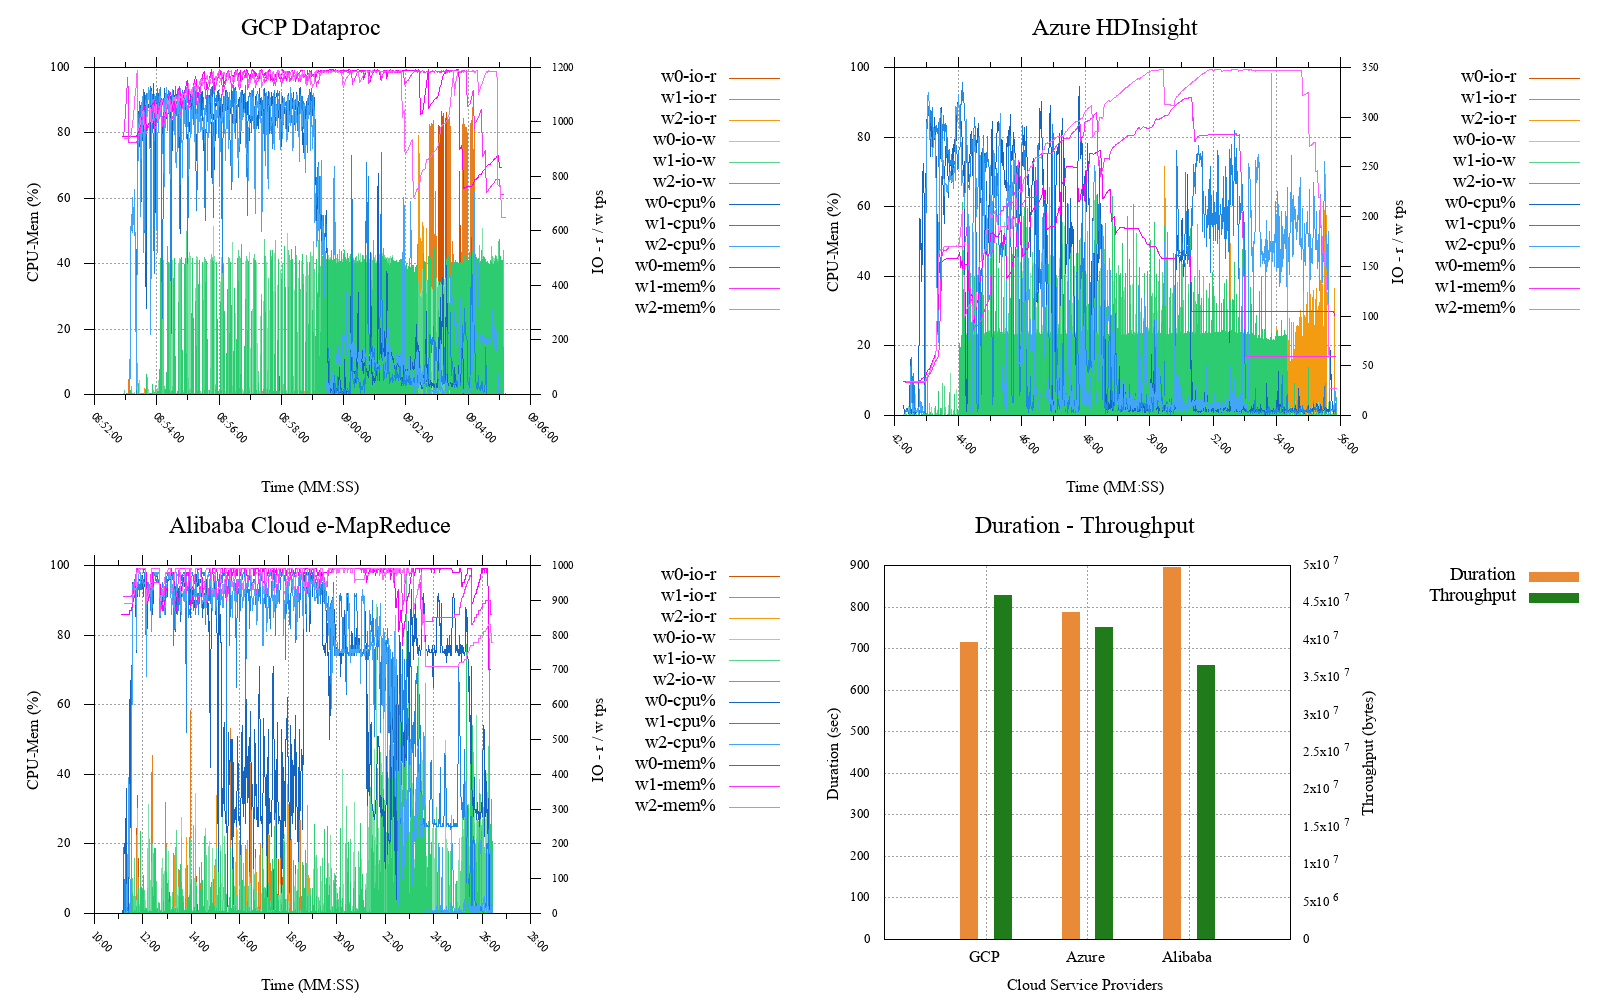
\includegraphics[width=\textwidth]{uc1-srt-g-cmidt}
	\centering
\end{figure}

\begin{figure}[b]
	\caption{UC1 - Terasort (Huge; 320 MB)}
	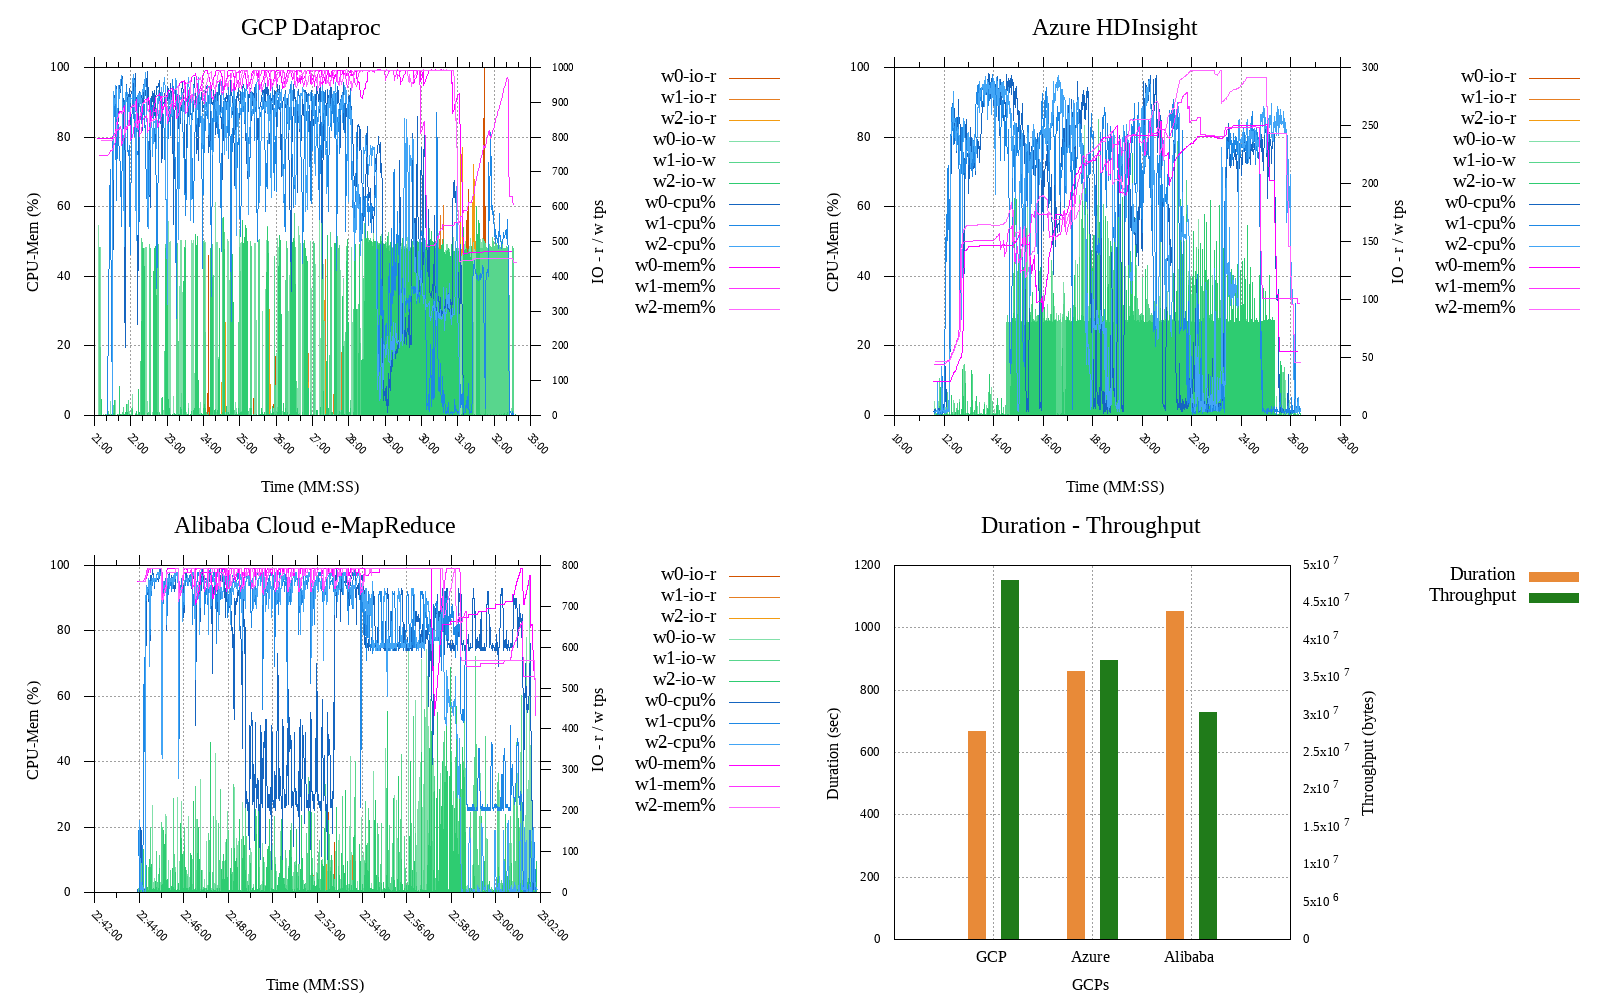
\includegraphics[width=\textwidth]{uc1-tera-h-cmidt}
	\centering
\end{figure}

\begin{figure}[b]
	\caption{UC1 - Terasort (Gigantic; 3.2 GB)}
	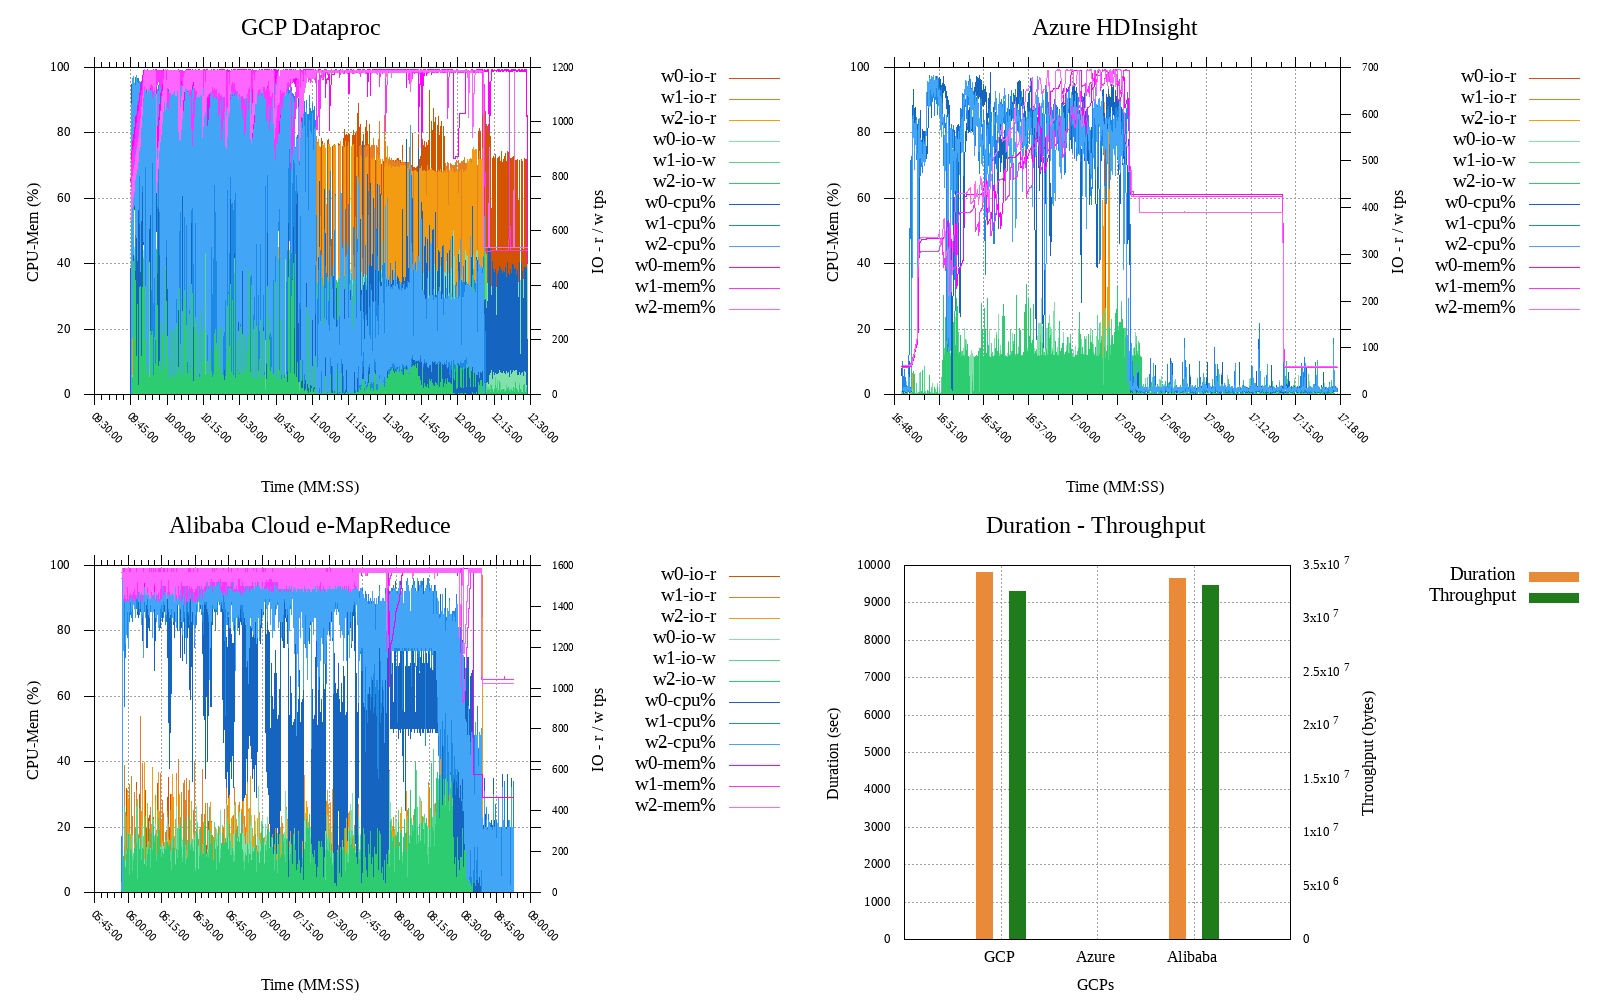
\includegraphics[width=\textwidth]{uc1-tera-g-cmidt}
	\centering
\end{figure}

\begin{figure}[b]
	\caption{UC1 - Wordcount (Huge; 32 GB)}
	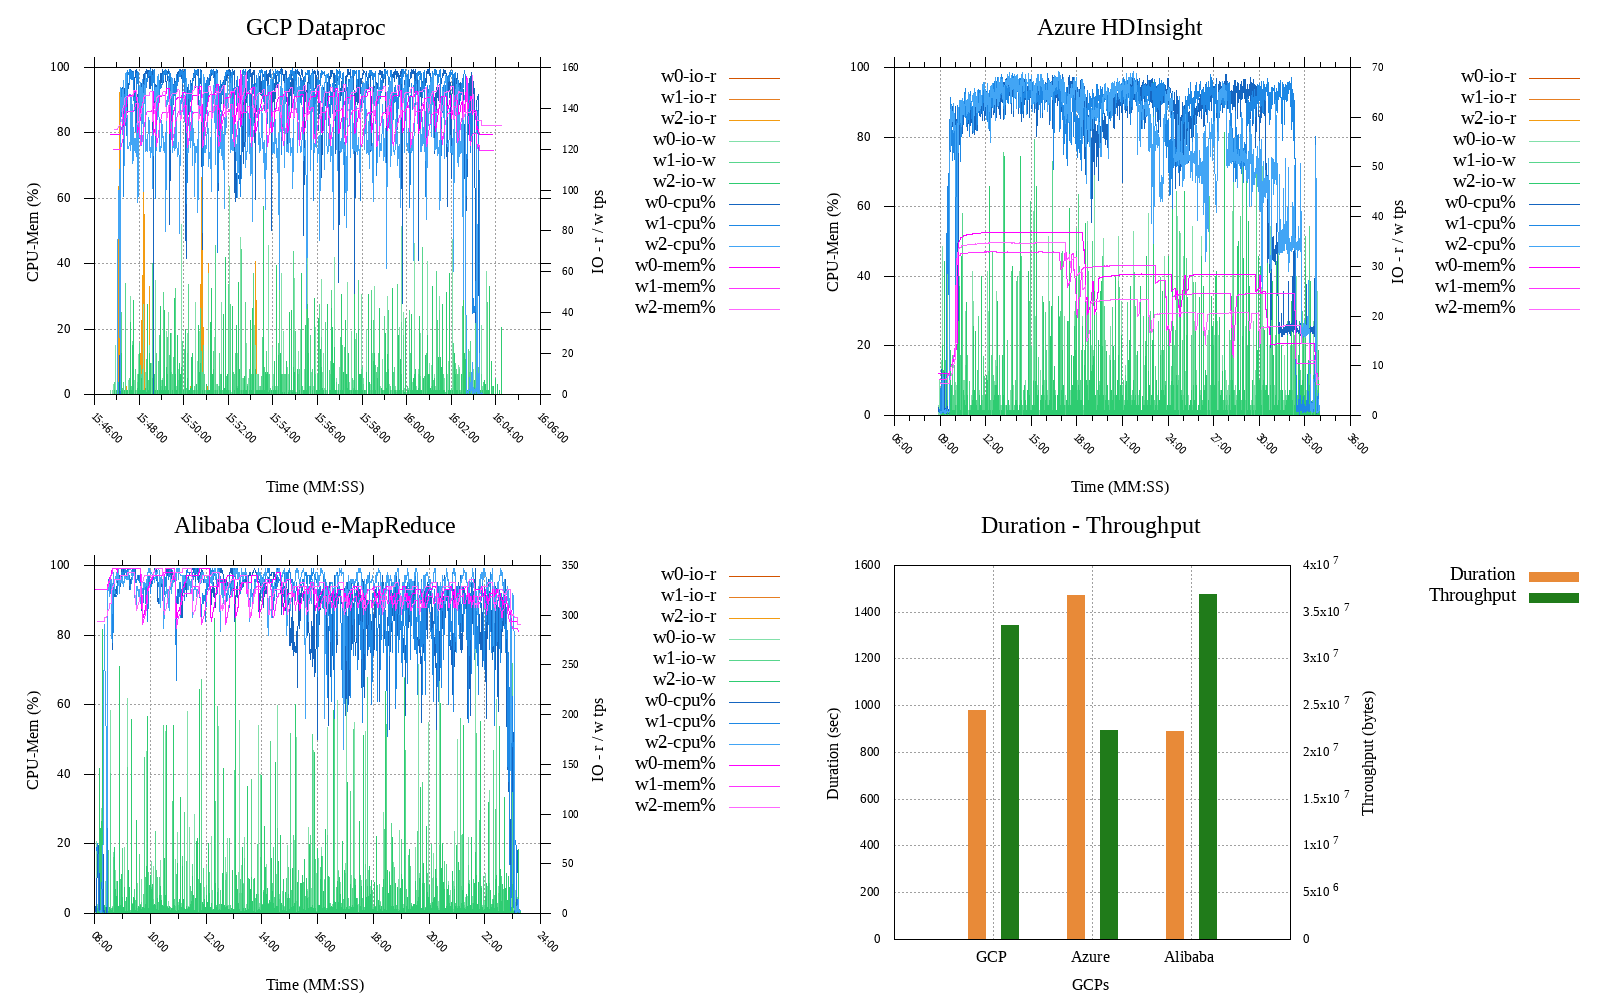
\includegraphics[width=\textwidth]{uc1-wrdcnt-h-cmidt}
	\centering
\end{figure}

\begin{figure}[b]
	\caption{UC1 - Wordcount (Gigantic; 320 GB)}
	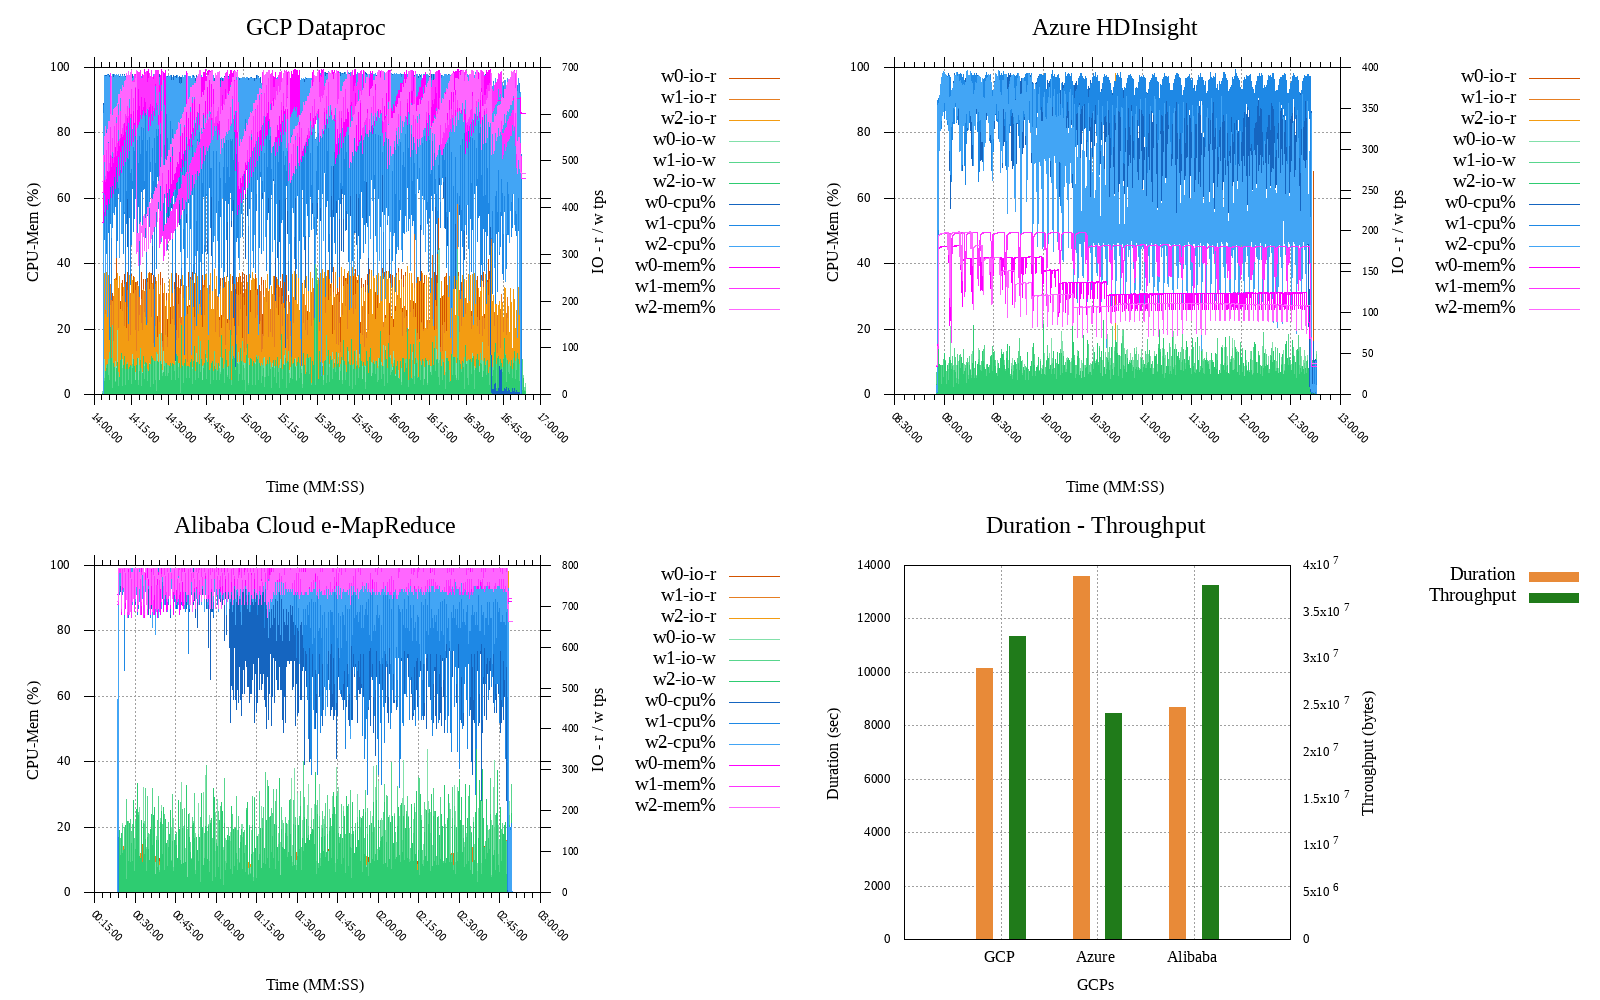
\includegraphics[width=\textwidth]{uc1-wrdcnt-g-cmidt}
	\centering
\end{figure}

\begin{figure}[b]
	\caption{UC1 - Dfsioe-read (Huge; No of Files: 256, File size: 100 MB)}
	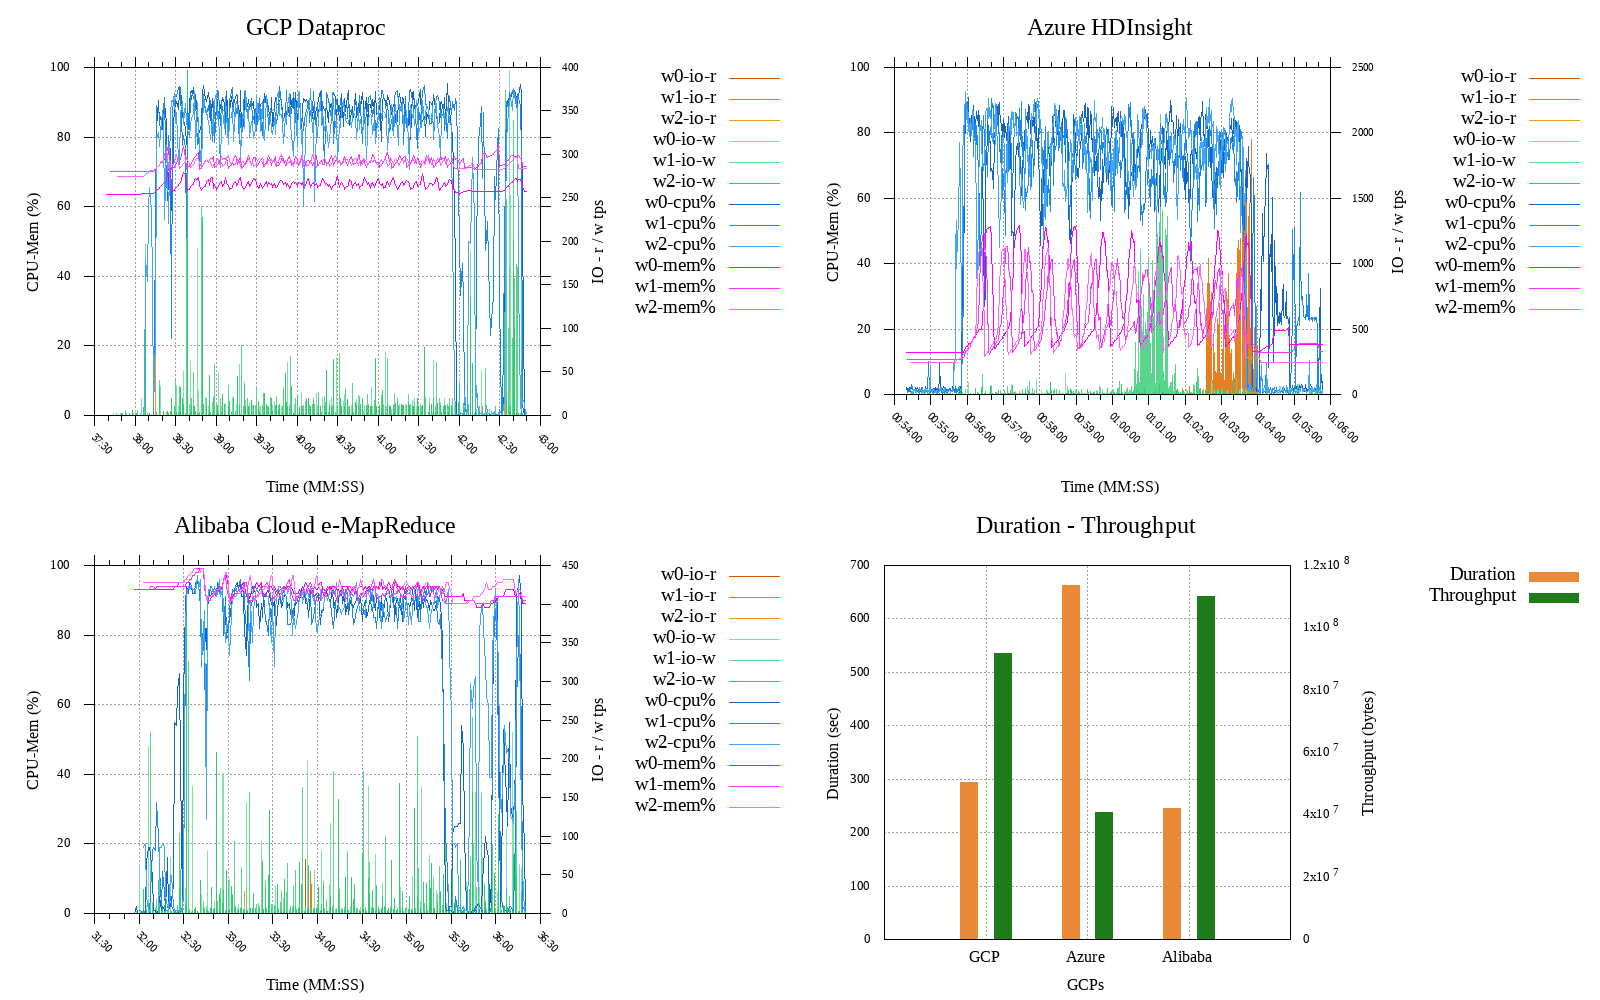
\includegraphics[width=\textwidth]{uc1-dfsioer-h-cmidt}
	\centering
\end{figure}

\begin{figure}[b]
	\caption{UC1 - Dfsioe-read (Gigantic; No of Files: 512, File size: 400 MB)}
	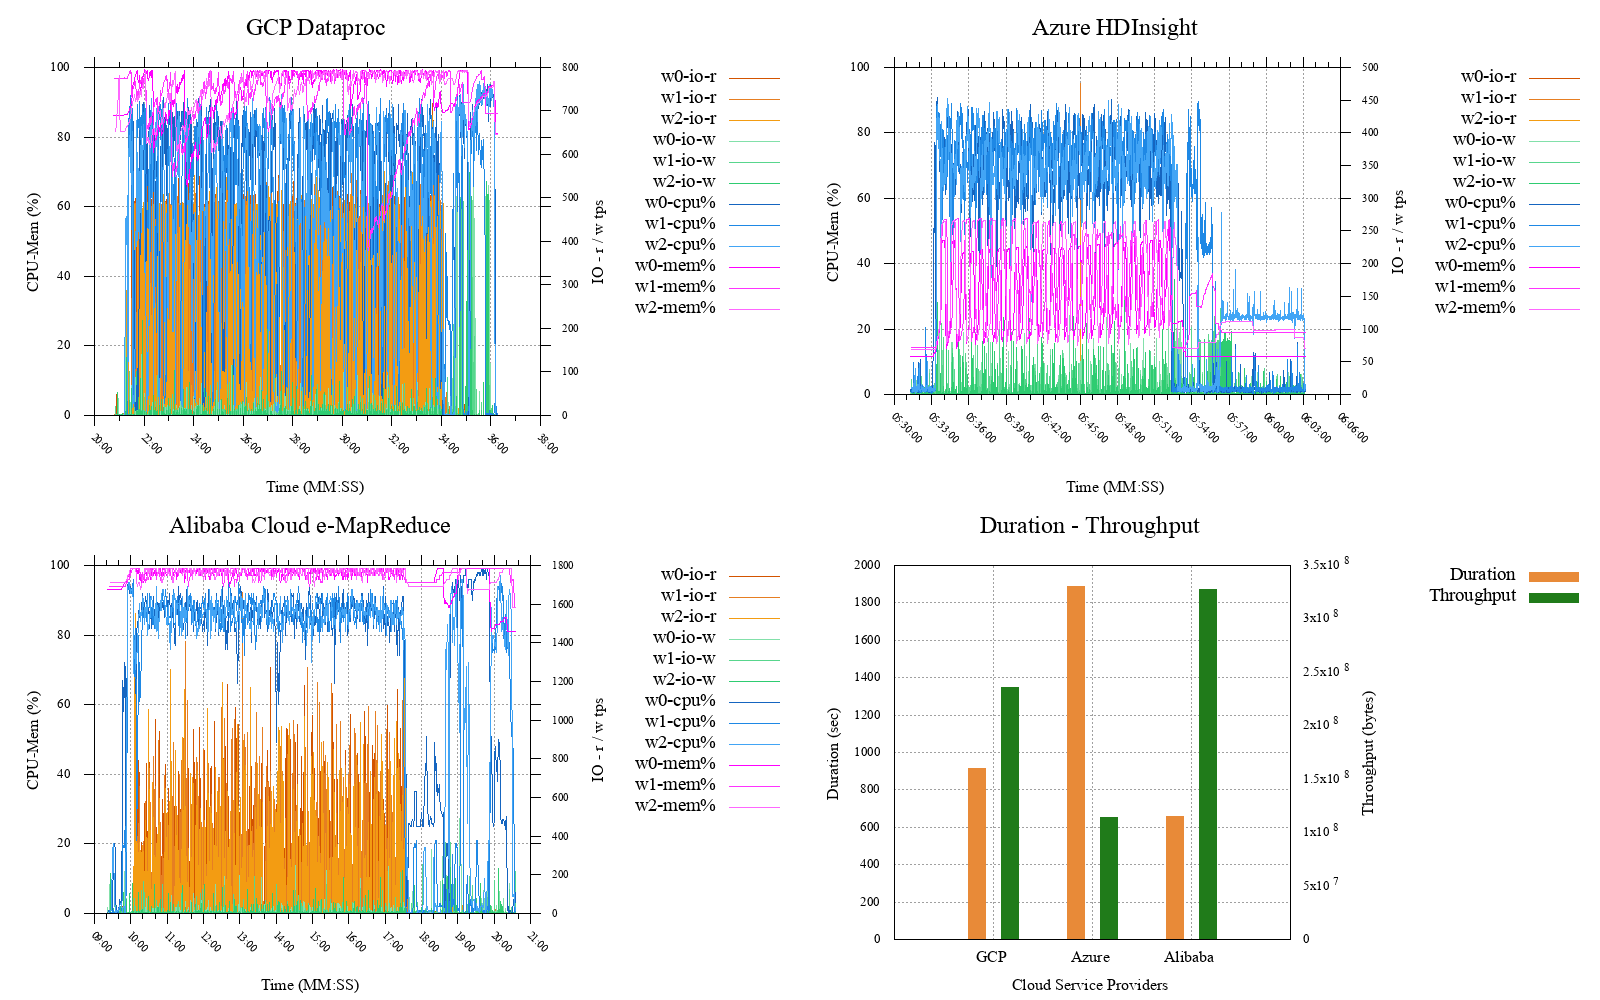
\includegraphics[width=\textwidth]{uc1-dfsioer-g-cmidt}
	\centering
\end{figure}

\begin{figure}[b]
	\caption{UC1 - Dfsioe-write (Huge; No of Files: 256, File size: 100 MB)}
	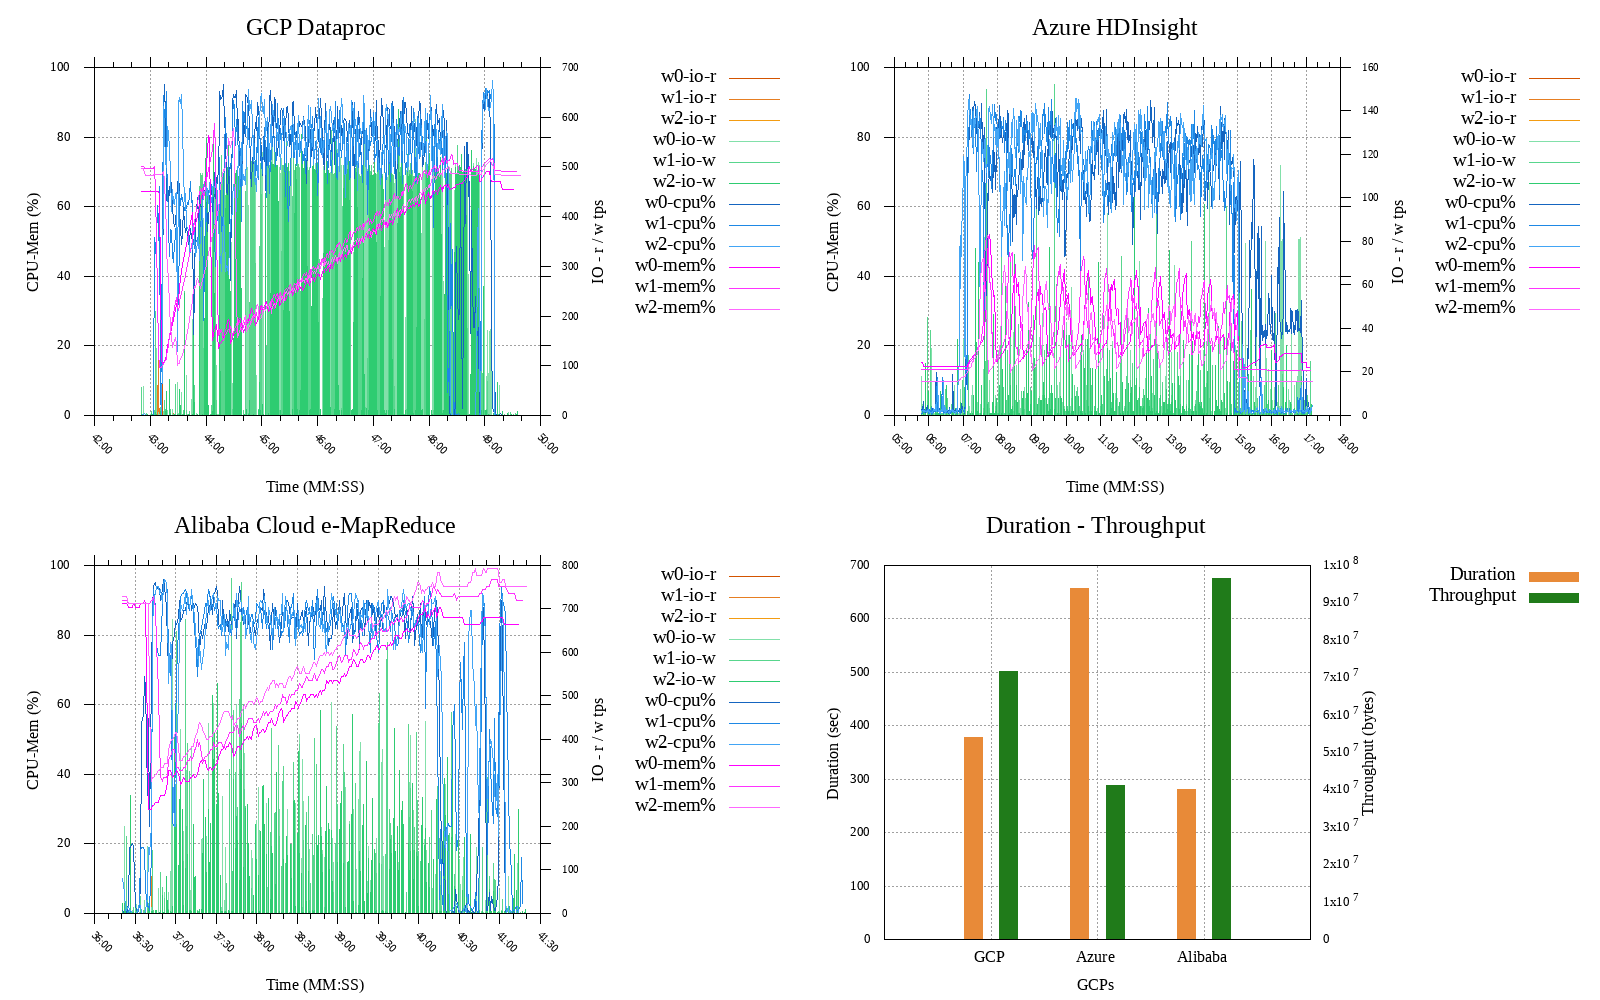
\includegraphics[width=\textwidth]{uc1-dfsioew-h-cmidt}
	\centering
\end{figure}

\begin{figure}[b]
	\caption{UC1 - Dfsioe-write (Gigantic; No of Files: 512, File size: 400 MB)}
	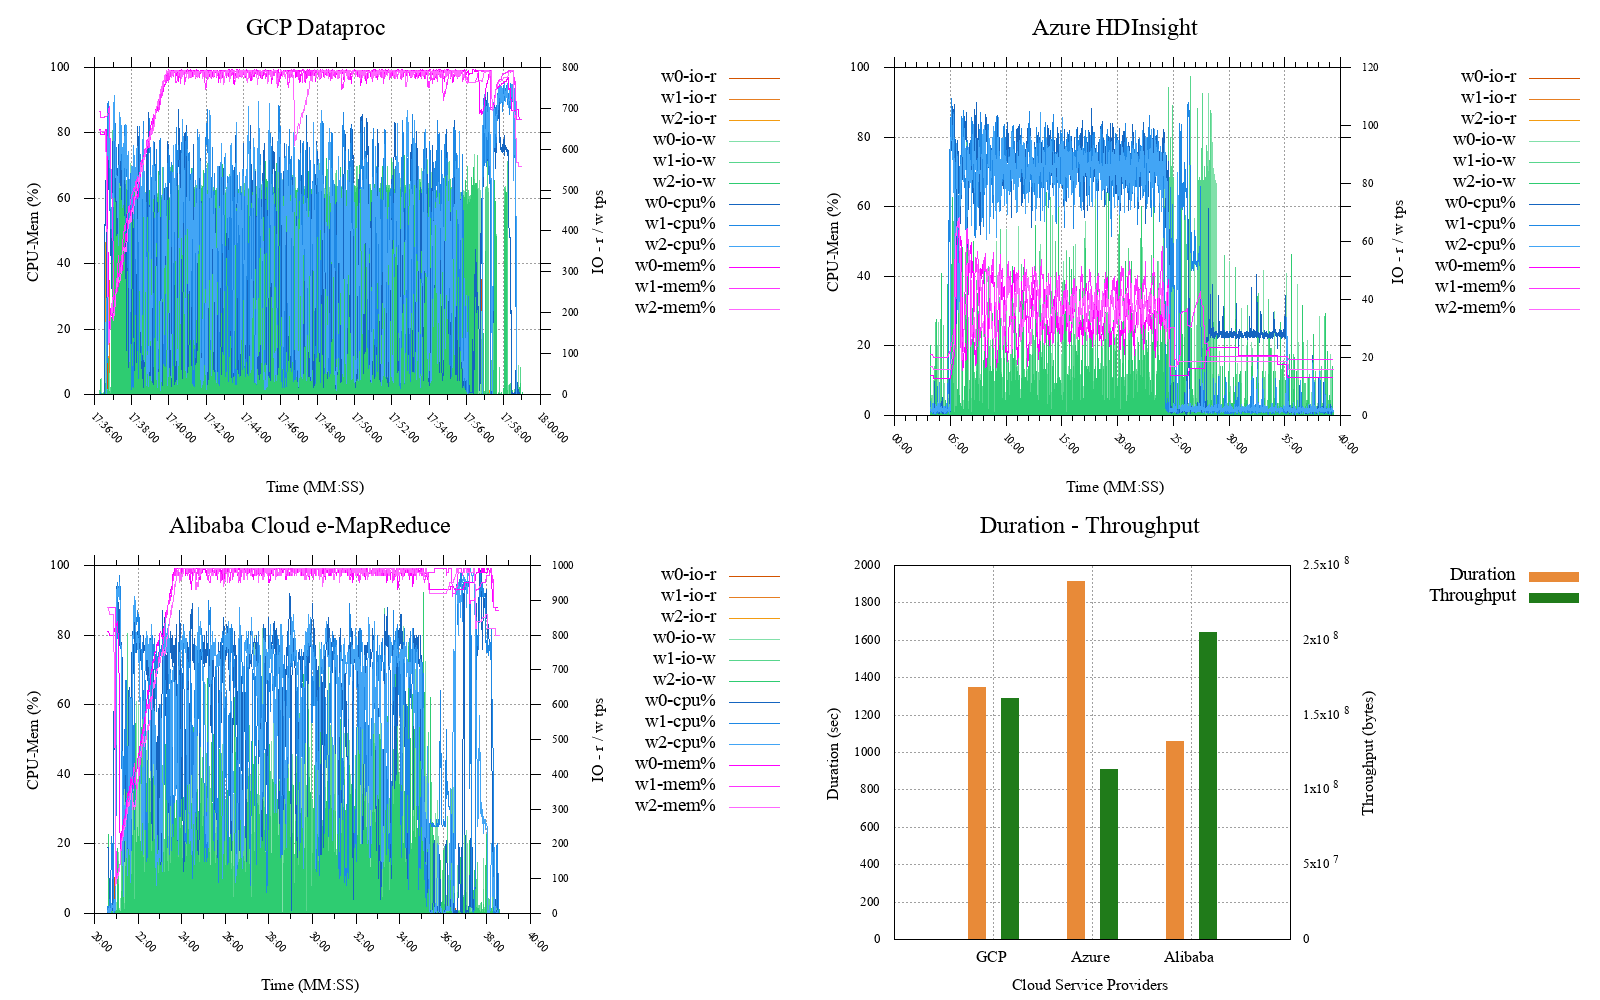
\includegraphics[width=\textwidth]{uc1-dfsioew-g-cmidt}
	\centering
\end{figure}

\begin{figure}[b]
	\caption{UC1 - Scan (Huge; USERVISITS: 10,000,000 PAGES: 1,200,000)}
	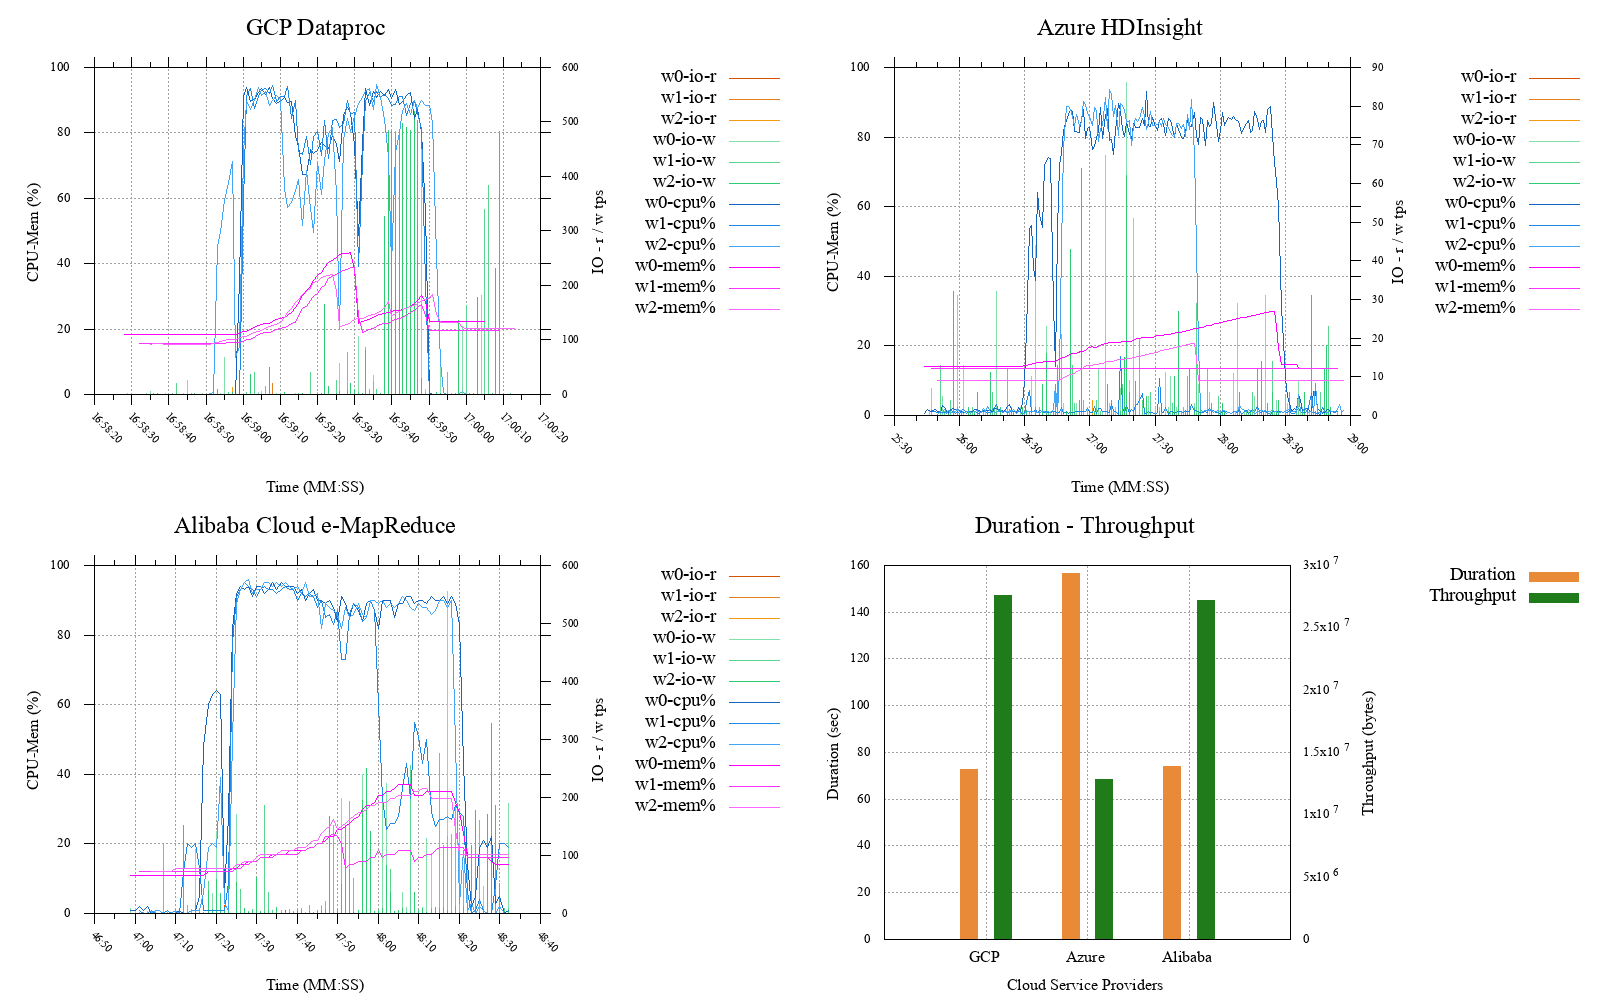
\includegraphics[width=\textwidth]{uc1-scan-h-cmidt}
	\centering
\end{figure}

\begin{figure}[b]
	\caption{UC1 - Scan (Gigantic; USERVISITS: 100,000,000 PAGES: 12,000,000)}
	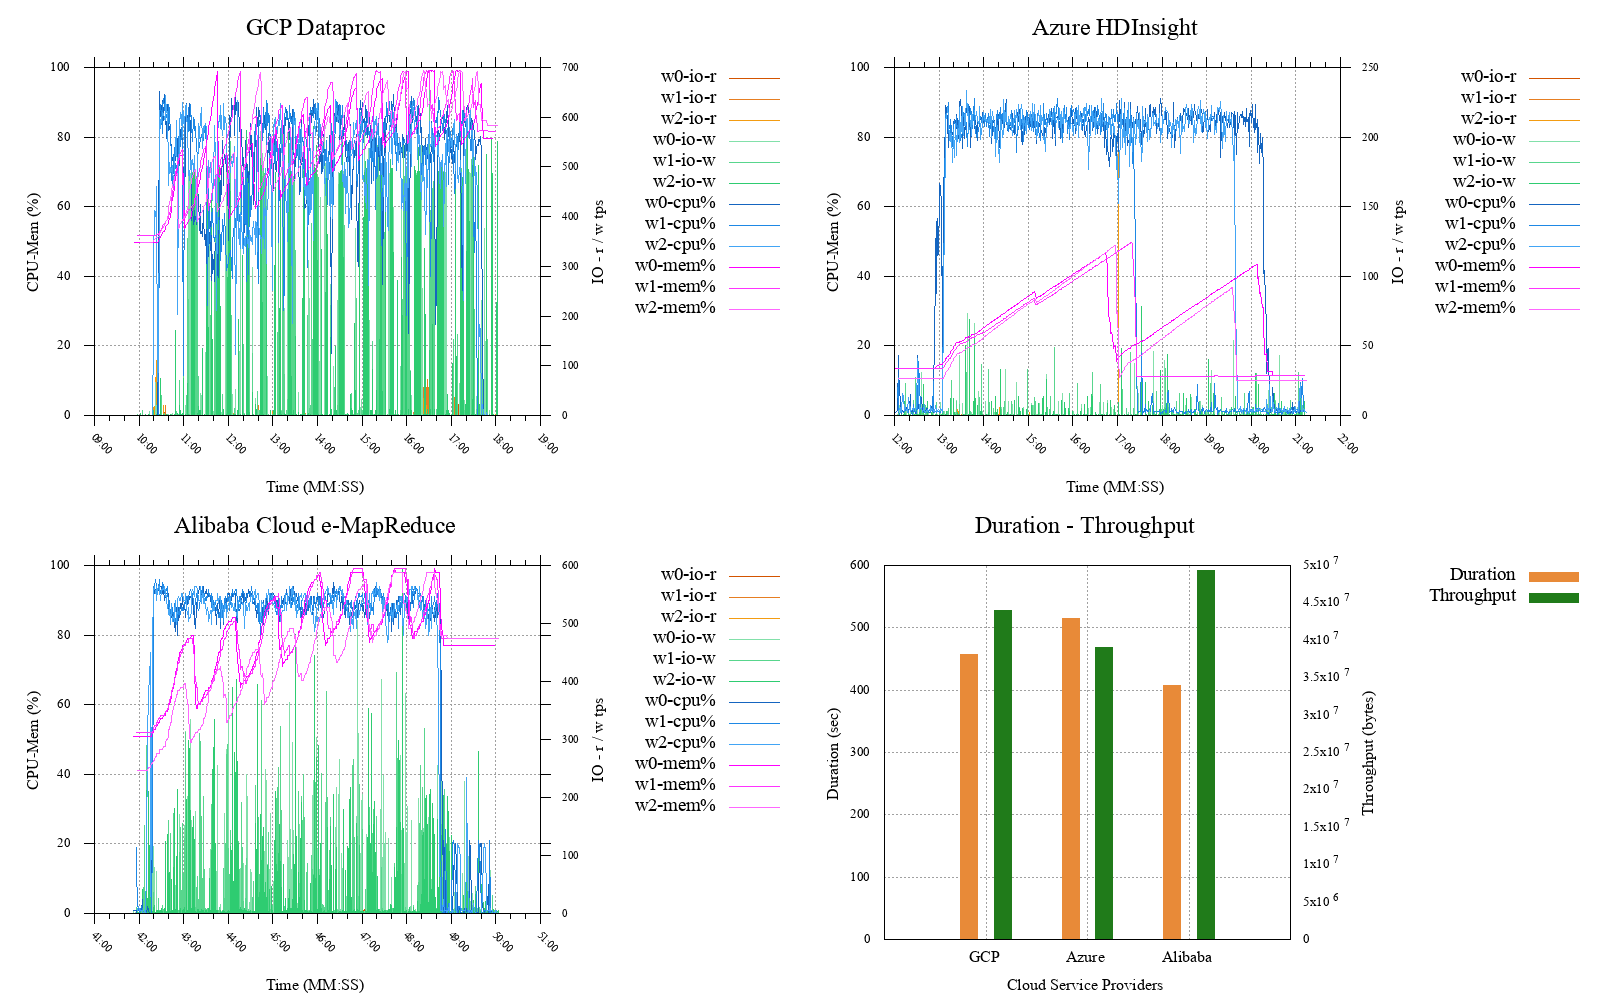
\includegraphics[width=\textwidth]{uc1-scan-g-cmidt}
	\centering
\end{figure}

\begin{figure}[b]
	\caption{UC1 - Join (Huge; USERVISITS: 10,000,000 PAGES: 1,200,000)}
	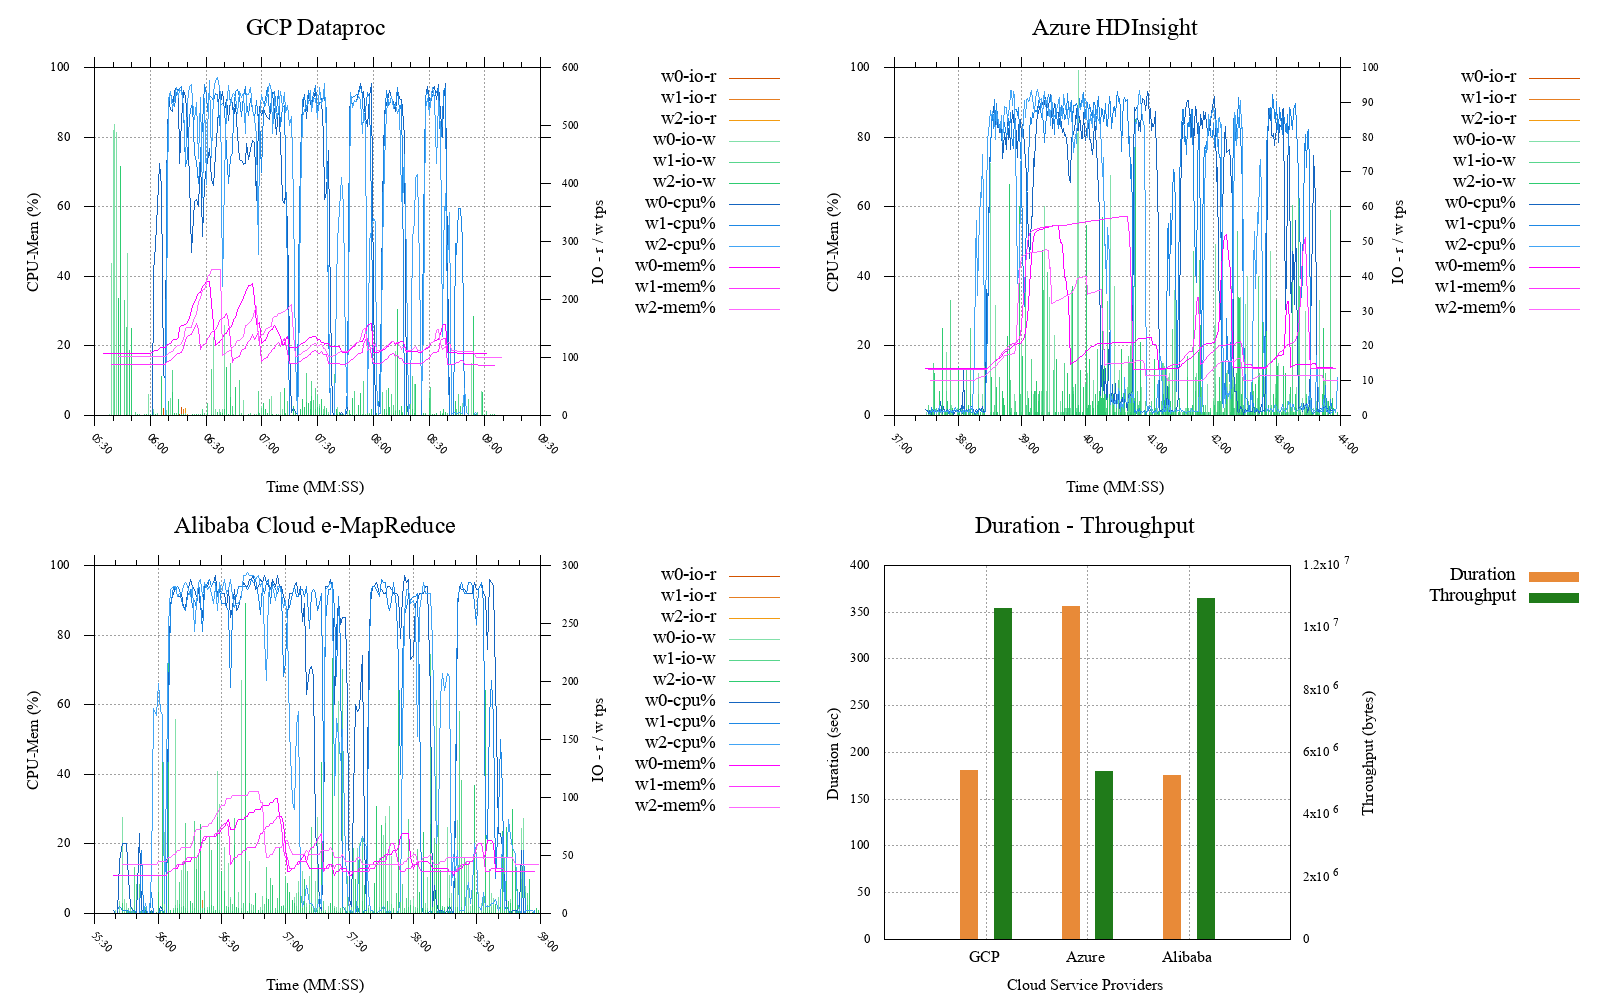
\includegraphics[width=\textwidth]{uc1-join-h-cmidt}
	\centering
\end{figure}

\begin{figure}[b]
	\caption{UC1 - Join (Gigantic; USERVISITS: 100,000,000 PAGES: 12,000,000)}
	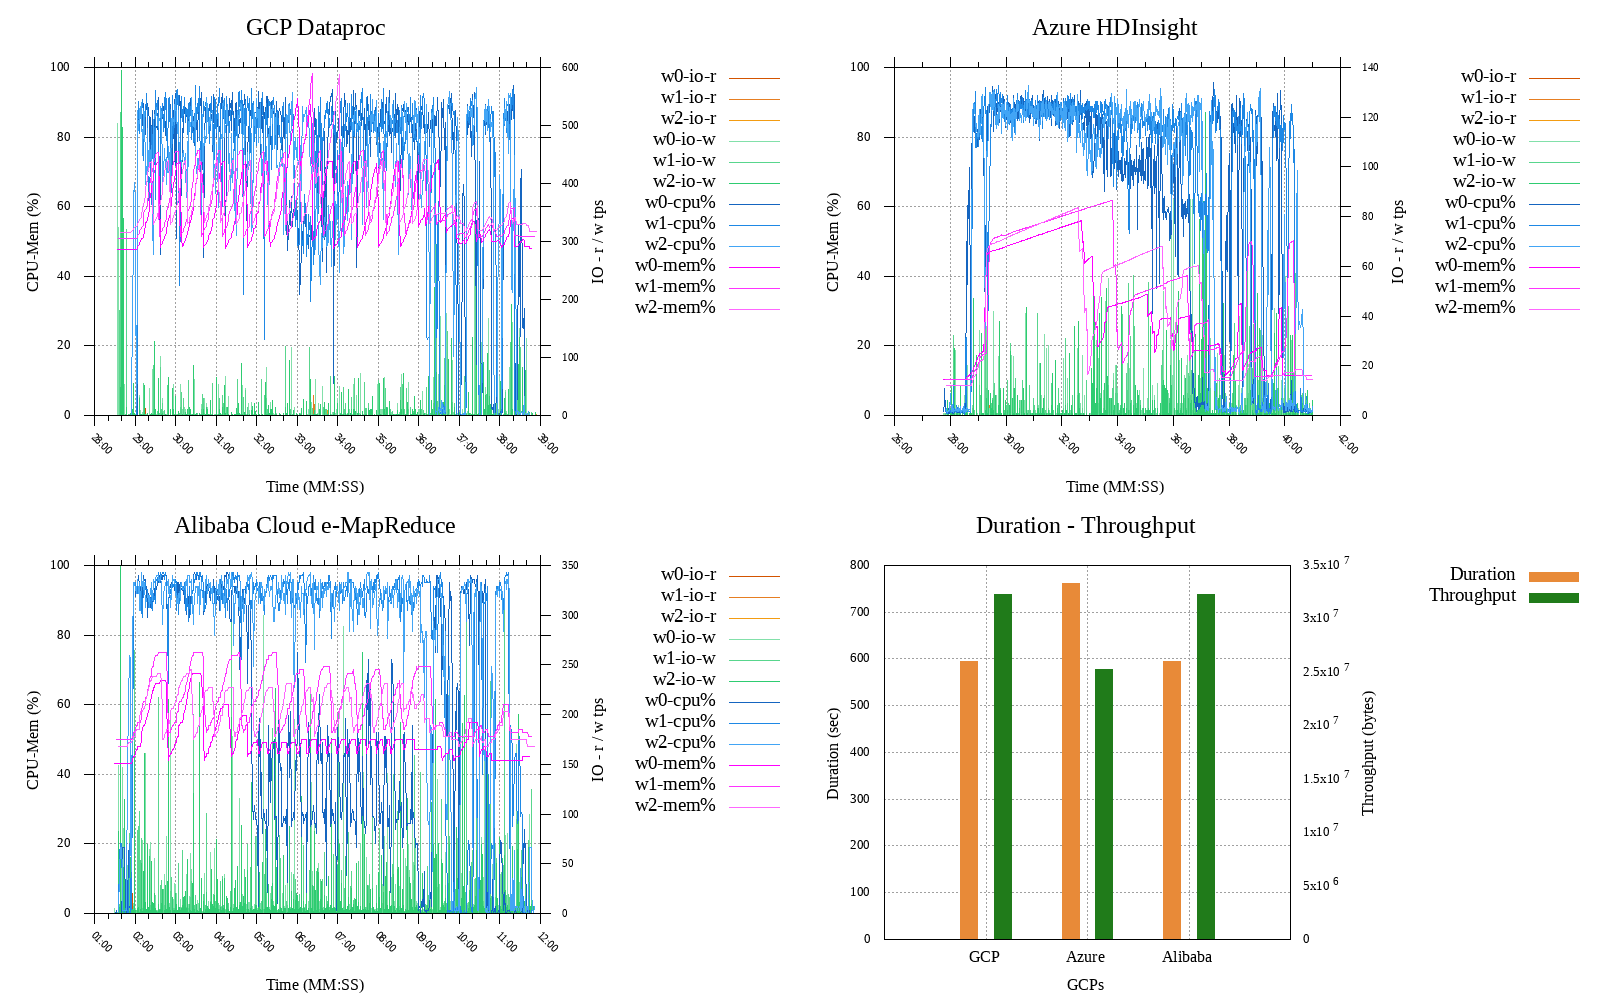
\includegraphics[width=\textwidth]{uc1-join-g-cmidt}
	\centering
\end{figure}

\begin{figure}[b]
	\caption{UC1 - Aggregation (Huge; USERVISITS: 10,000,000 PAGES: 1,200,000)}
	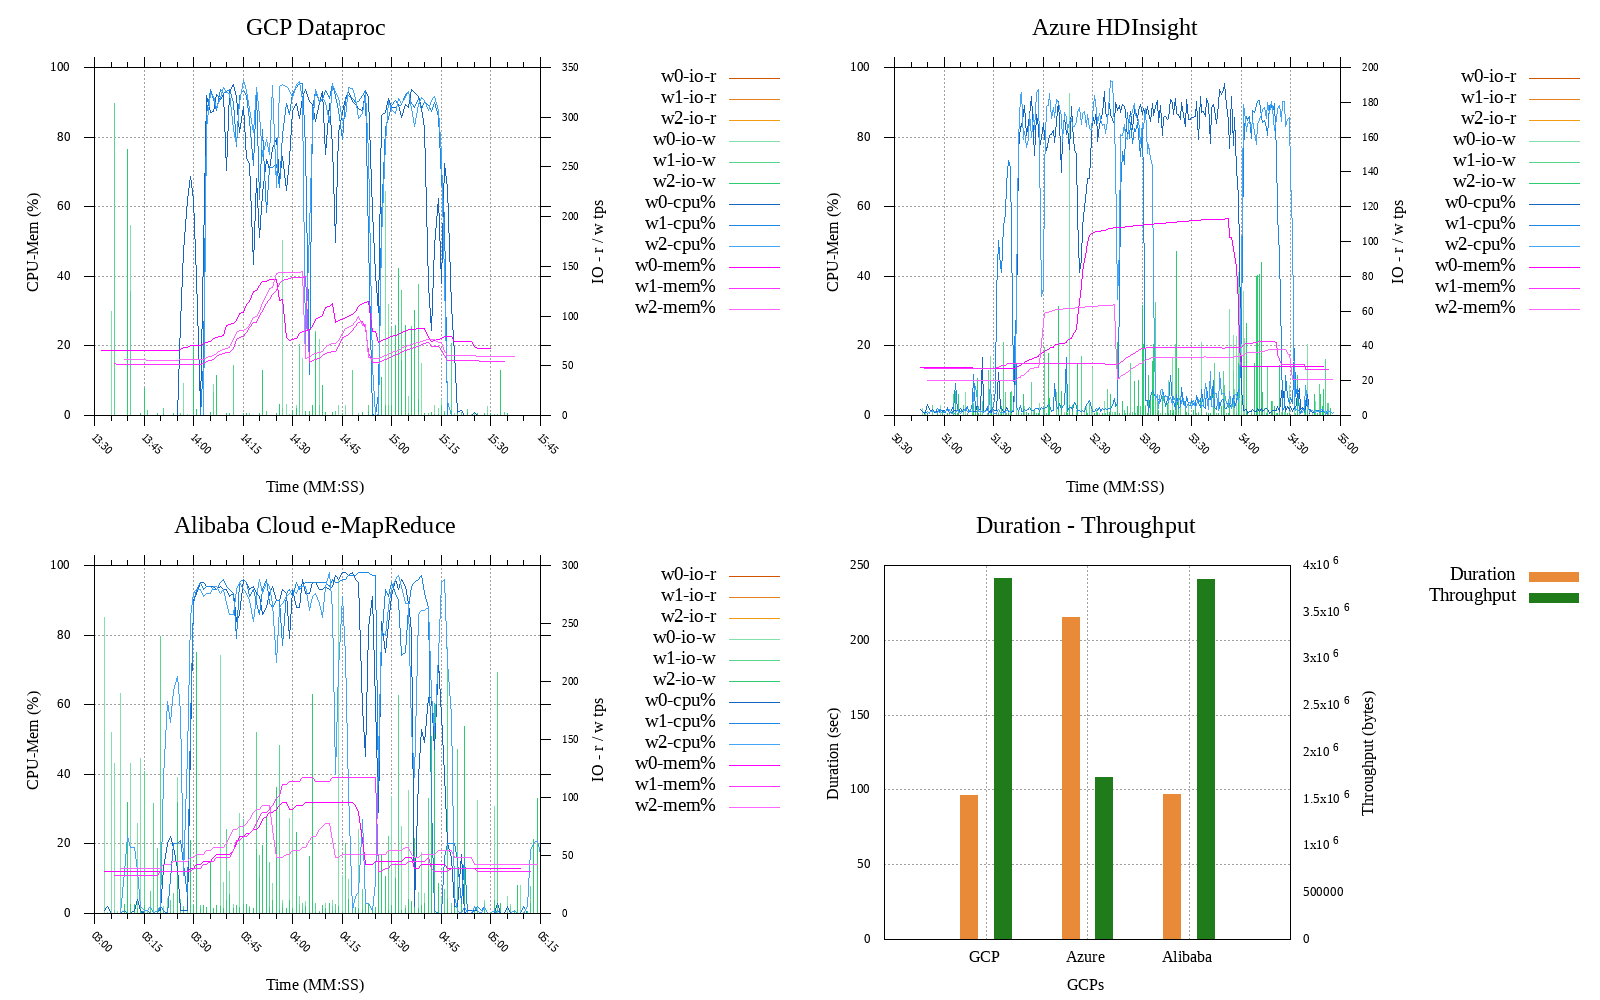
\includegraphics[width=\textwidth]{uc1-aggreg-h-cmidt}
	\centering
\end{figure}

\begin{figure}[b]
	\caption{UC1 - Aggregation (Gigantic; USERVISITS: 100,000,000 PAGES: 12,000,000)}
	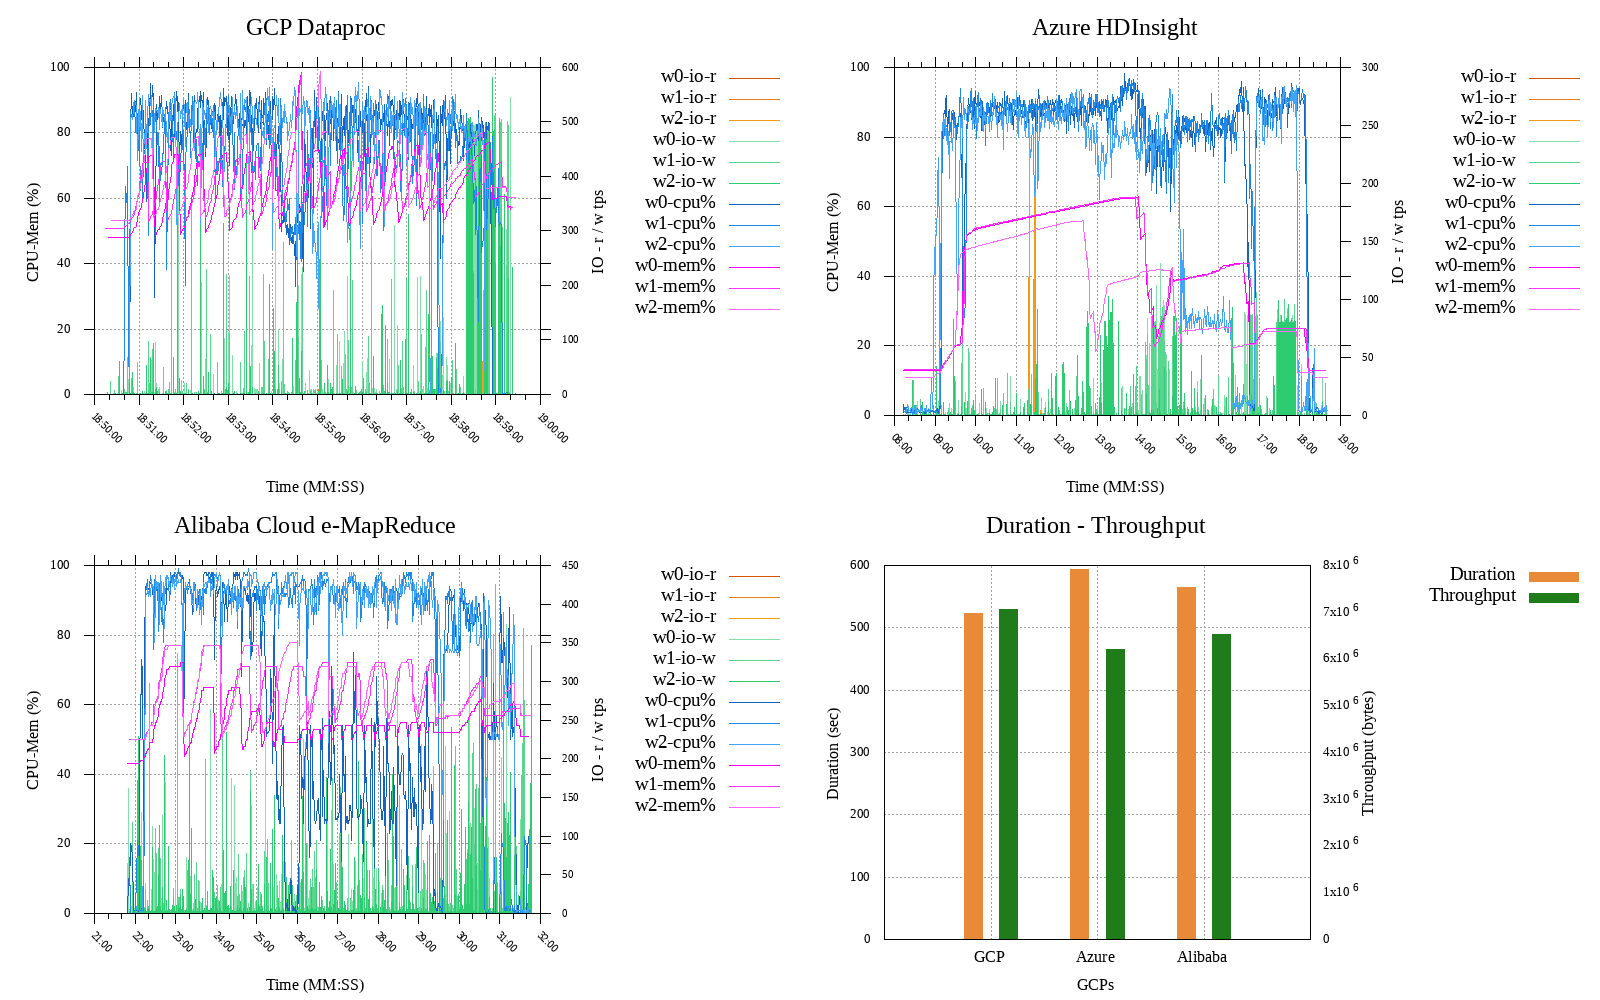
\includegraphics[width=\textwidth]{uc1-aggreg-g-cmidt}
	\centering
\end{figure}

\begin{figure}[b]
	\caption{UC1 - Bayes (Huge; PAGES: 500,000 CLASSES: 100 NGRAMS: 2)}
	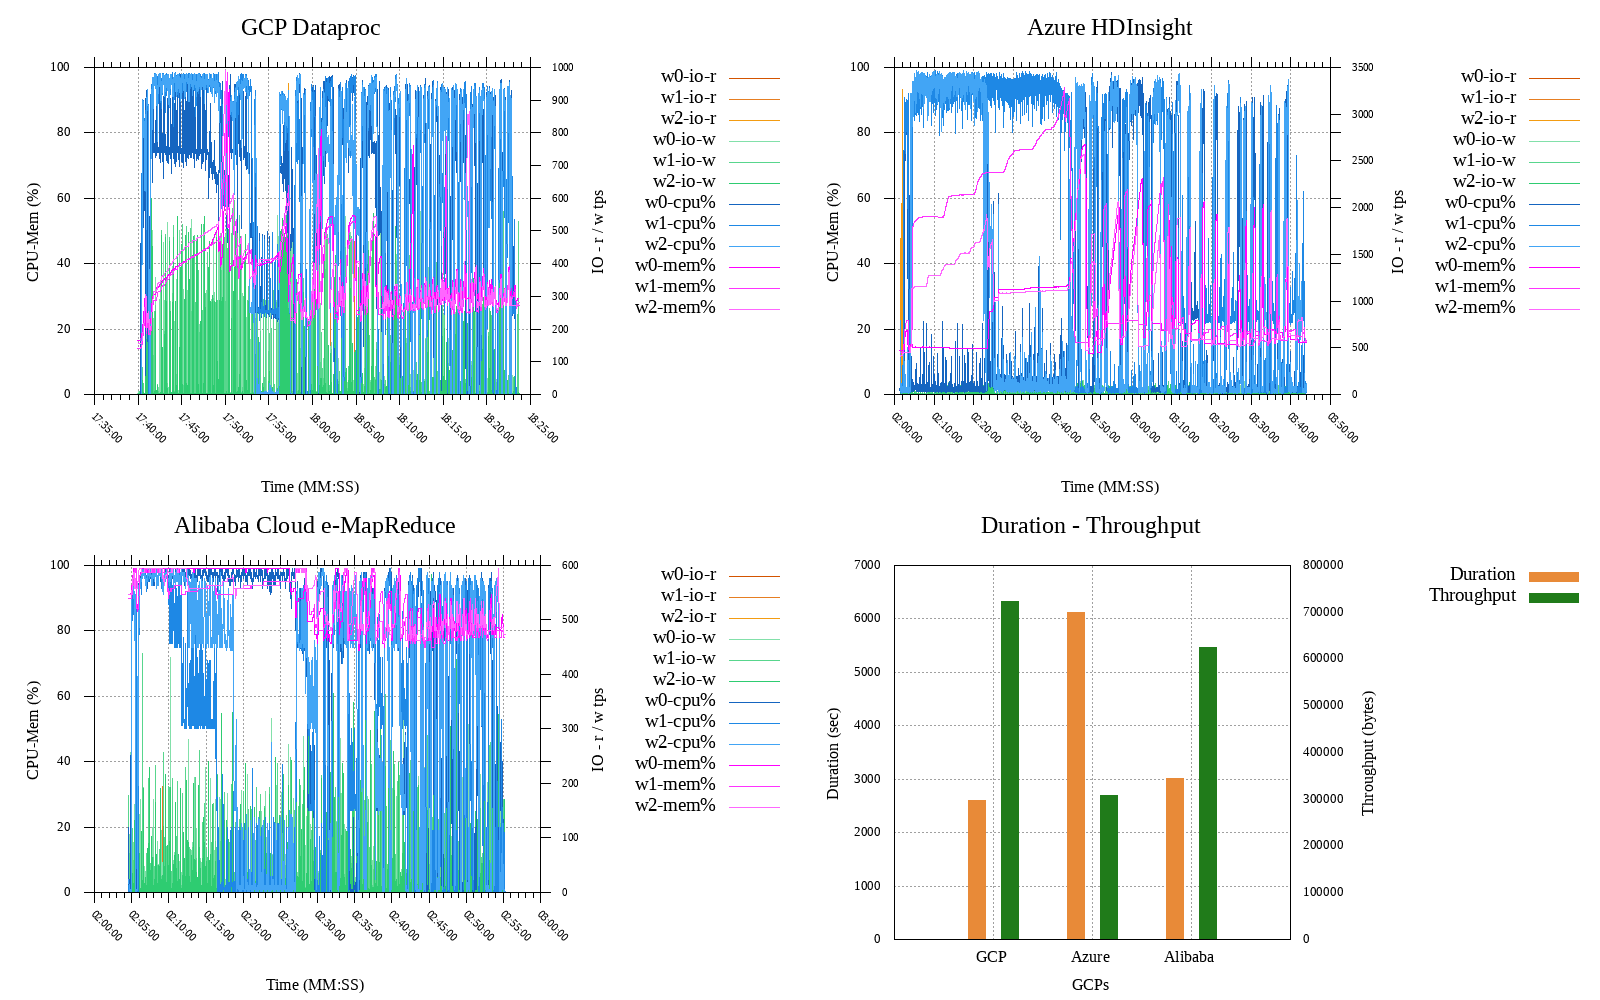
\includegraphics[width=\textwidth]{uc1-bayes-h-cmidt}
	\centering
\end{figure}

\begin{figure}[b]
	\caption{UC1 - Bayes (Gigantic; PAGES: 1,000,000 CLASSES: 100 NGRAMS: 2)}
	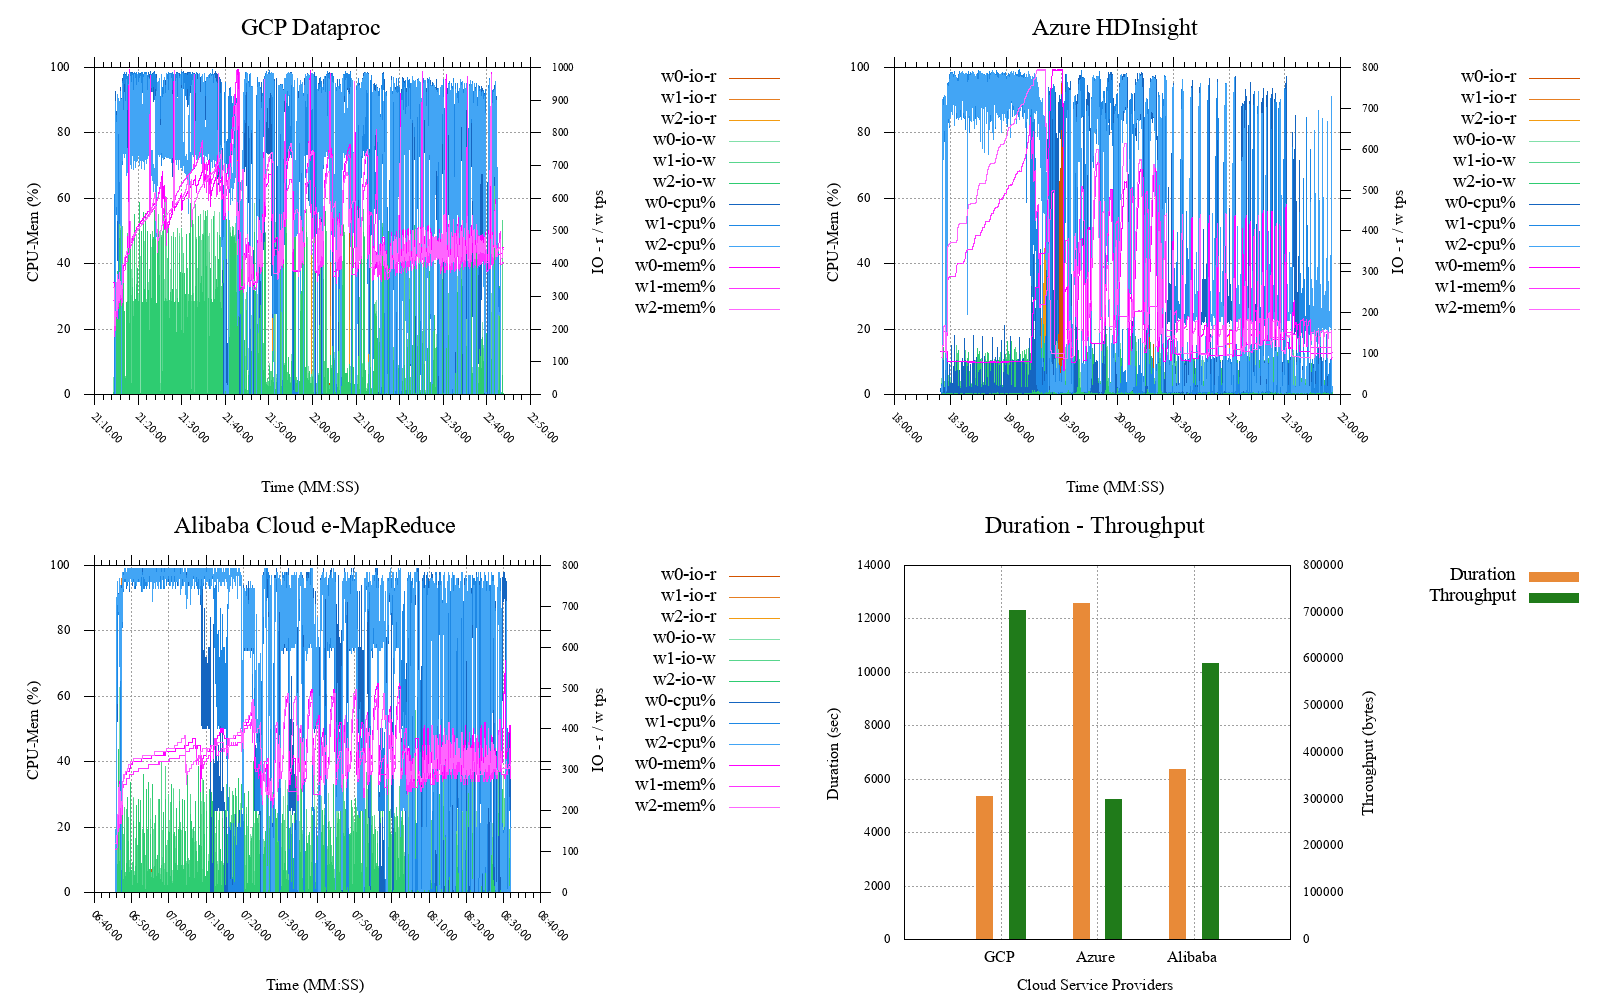
\includegraphics[width=\textwidth]{uc1-bayes-g-cmidt}
	\centering
\end{figure}

\begin{figure}[b]
	\caption{UC1 - Kmeans (Huge; CLUSTERS: 5 DIMENSIONS: 20 SAMPLES: 100,000,000 SAMP PER INPUT: 20,000,000 MAX IT: 5 K: 10 CONVERGEDIST: 0.5)}
	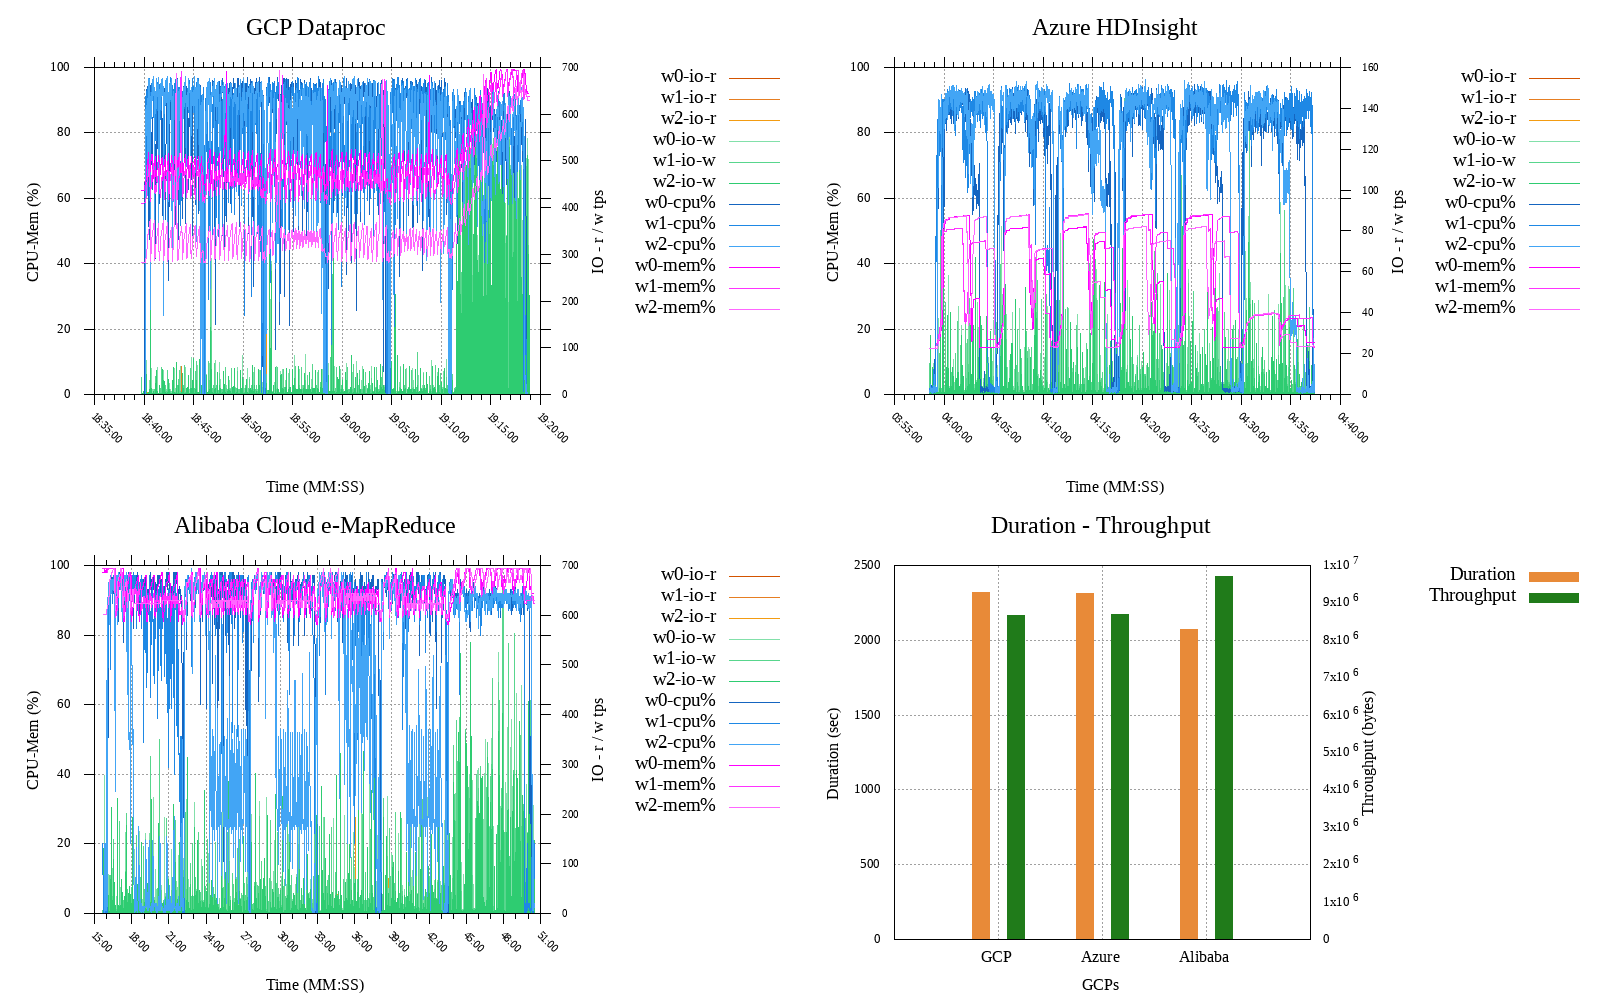
\includegraphics[width=\textwidth]{uc1-kmeans-h-cmidt}
	\centering
\end{figure}

\begin{figure}[b]
	\caption{UC1 - Kmeans (Gigantic; CLUSTERS: 5 DIMENSIONS: 20 SAMPLES: 200,000,000 SAMP PER INPUT: 40,000,000 MAX IT: 5 K: 10 CONVERGEDIST: 0.5)}
	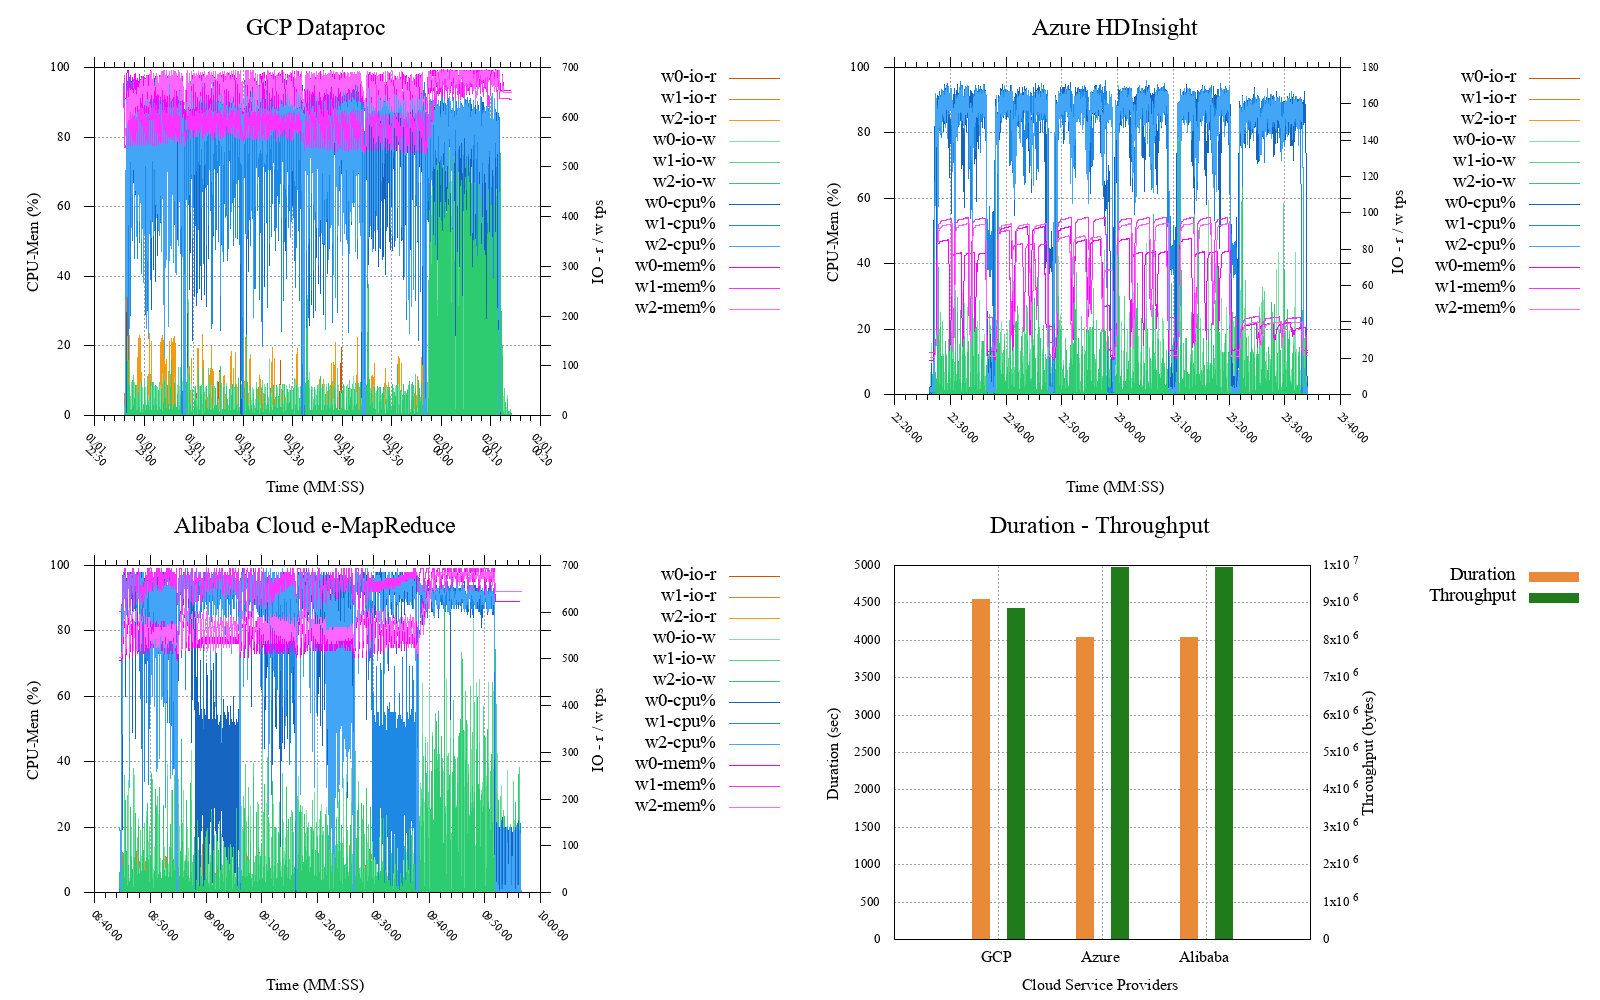
\includegraphics[width=\textwidth]{uc1-kmeans-g-cmidt}
	\centering
\end{figure}

\begin{figure}[b]
	\caption{UC1 - Pagerank (Huge; PAGES: 5,000,000 NUM ITERATIONS: 3 BLOCK: 0 BLOCK WIDTH: 16)}
	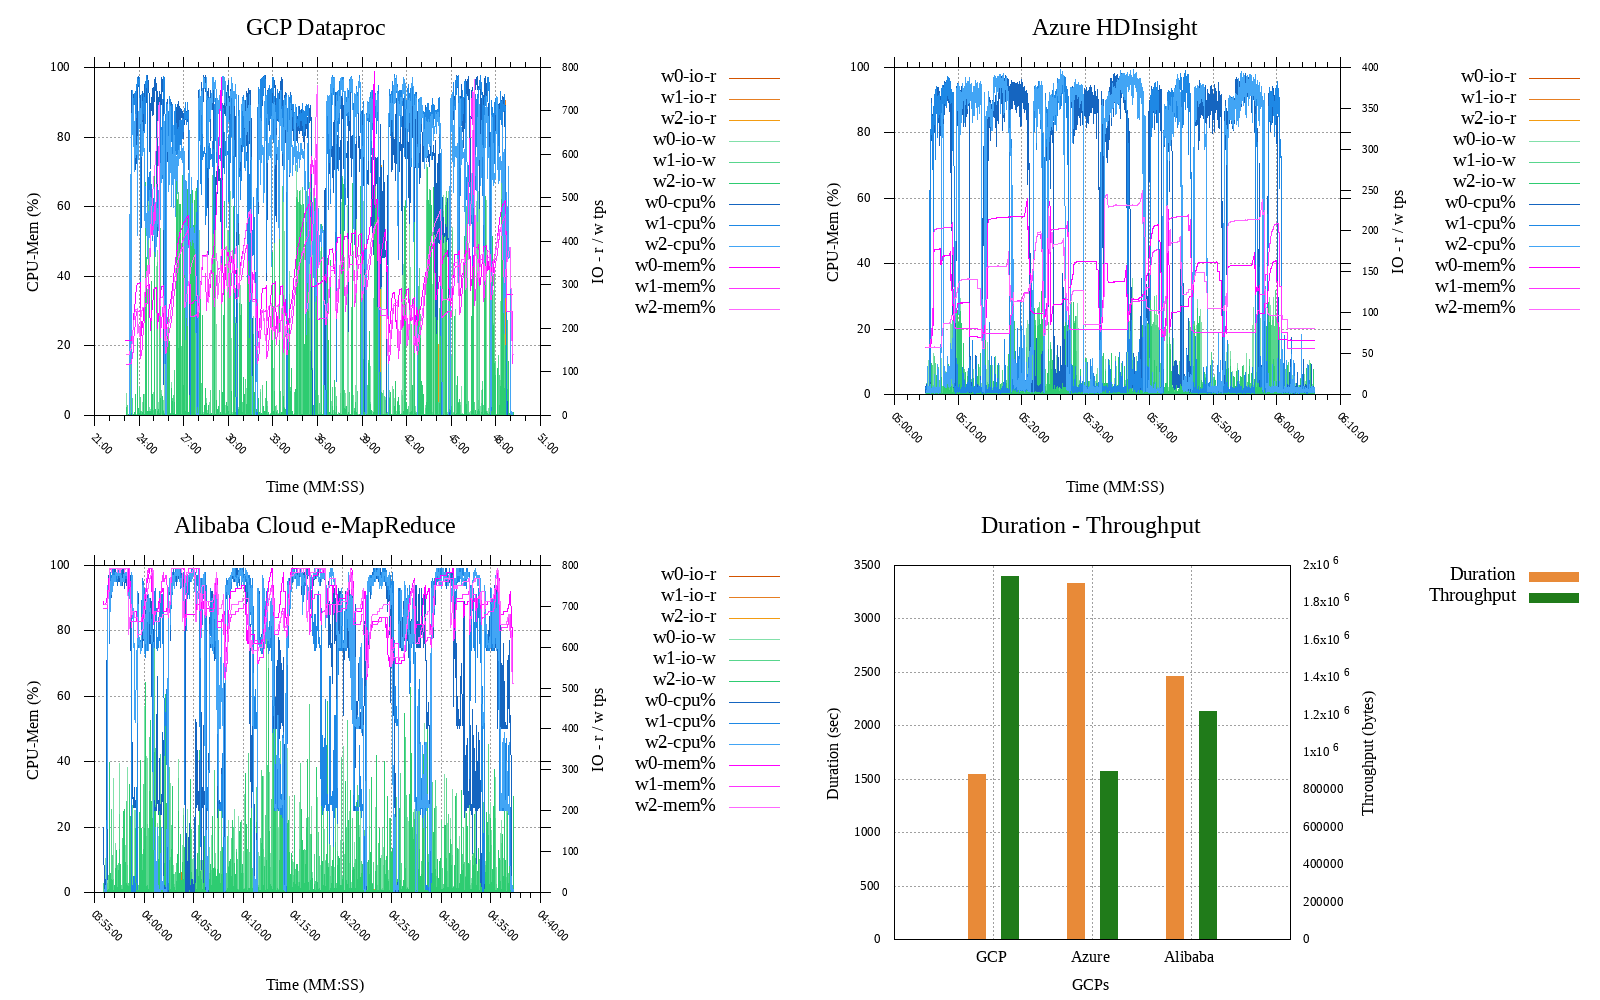
\includegraphics[width=\textwidth]{uc1-page-h-cmidt}
	\centering
\end{figure}

\begin{figure}[b]
	\caption{UC1 - Pagerank (Gigantic; PAGES: 30,000,000 NUM ITERATIONS: 3 BLOCK: 0 BLOCK WIDTH: 16)}
	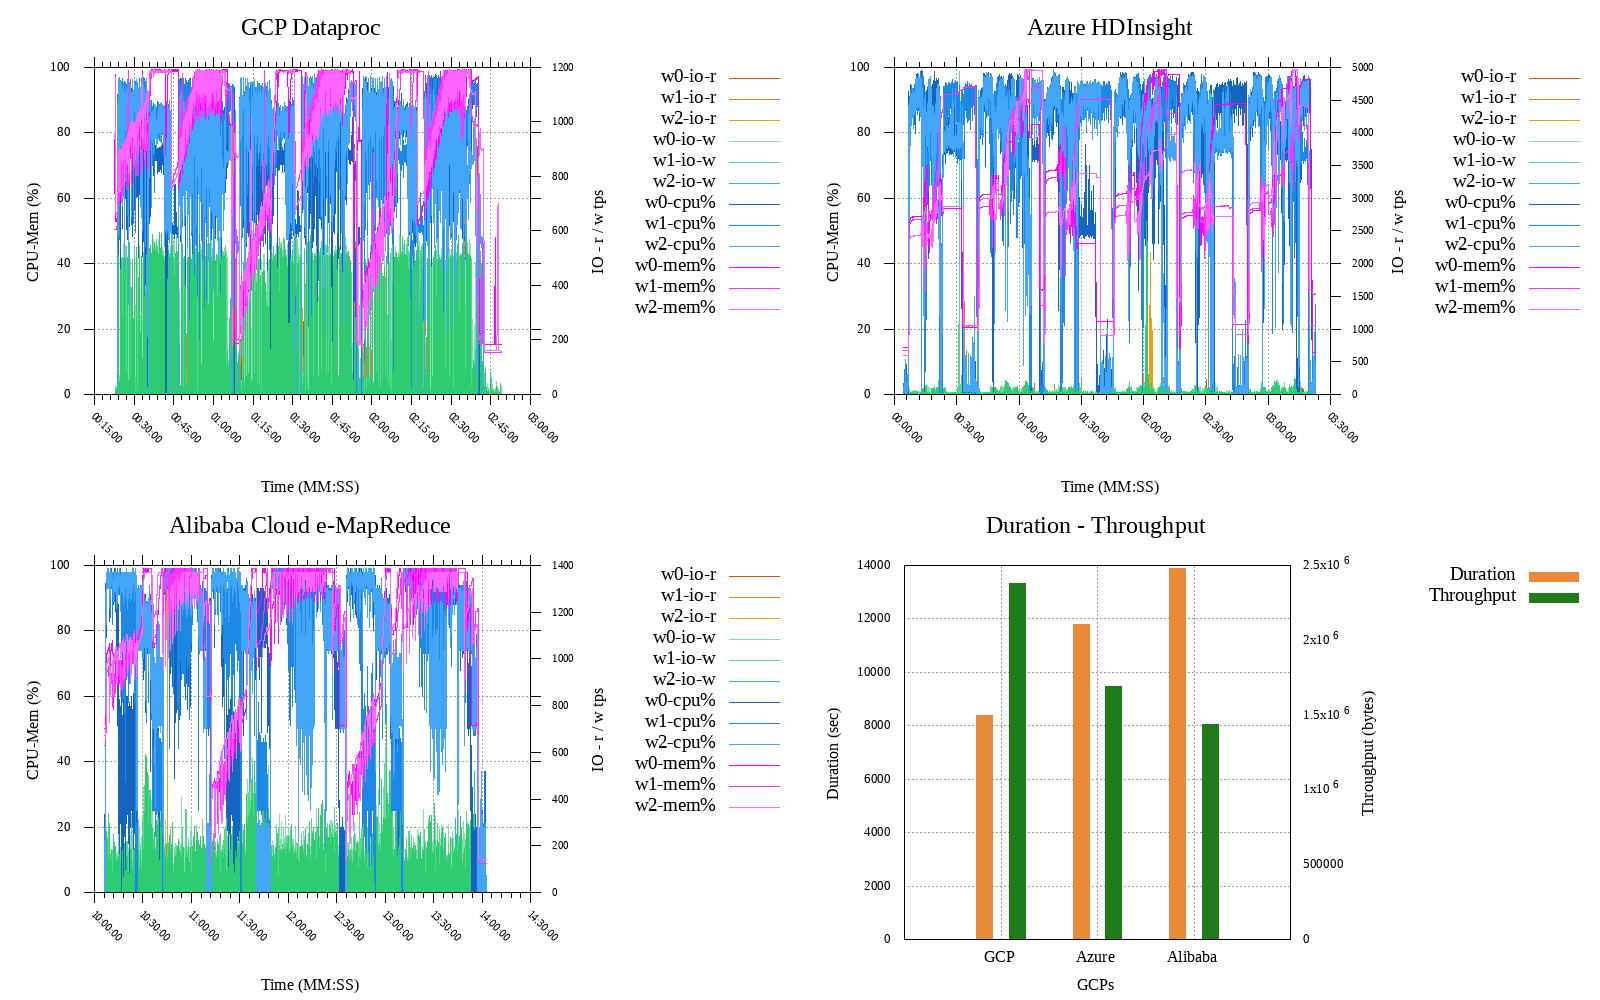
\includegraphics[width=\textwidth]{uc1-page-g-cmidt}
	\centering
\end{figure}

USE CASE 1: 

Sort - Tiny:

Sort - Small:

Sort - Large:

Sort - Huge:

Sort - Gigantic:

Wordcount - Tiny:

Wordcount - Small:

Wordcount - Large:

Wordcount - Huge:

Wordcount - Gigantic:

\begin{figure}[b]
	\caption{UC2 - Sort (Tiny; 32 KB)}
	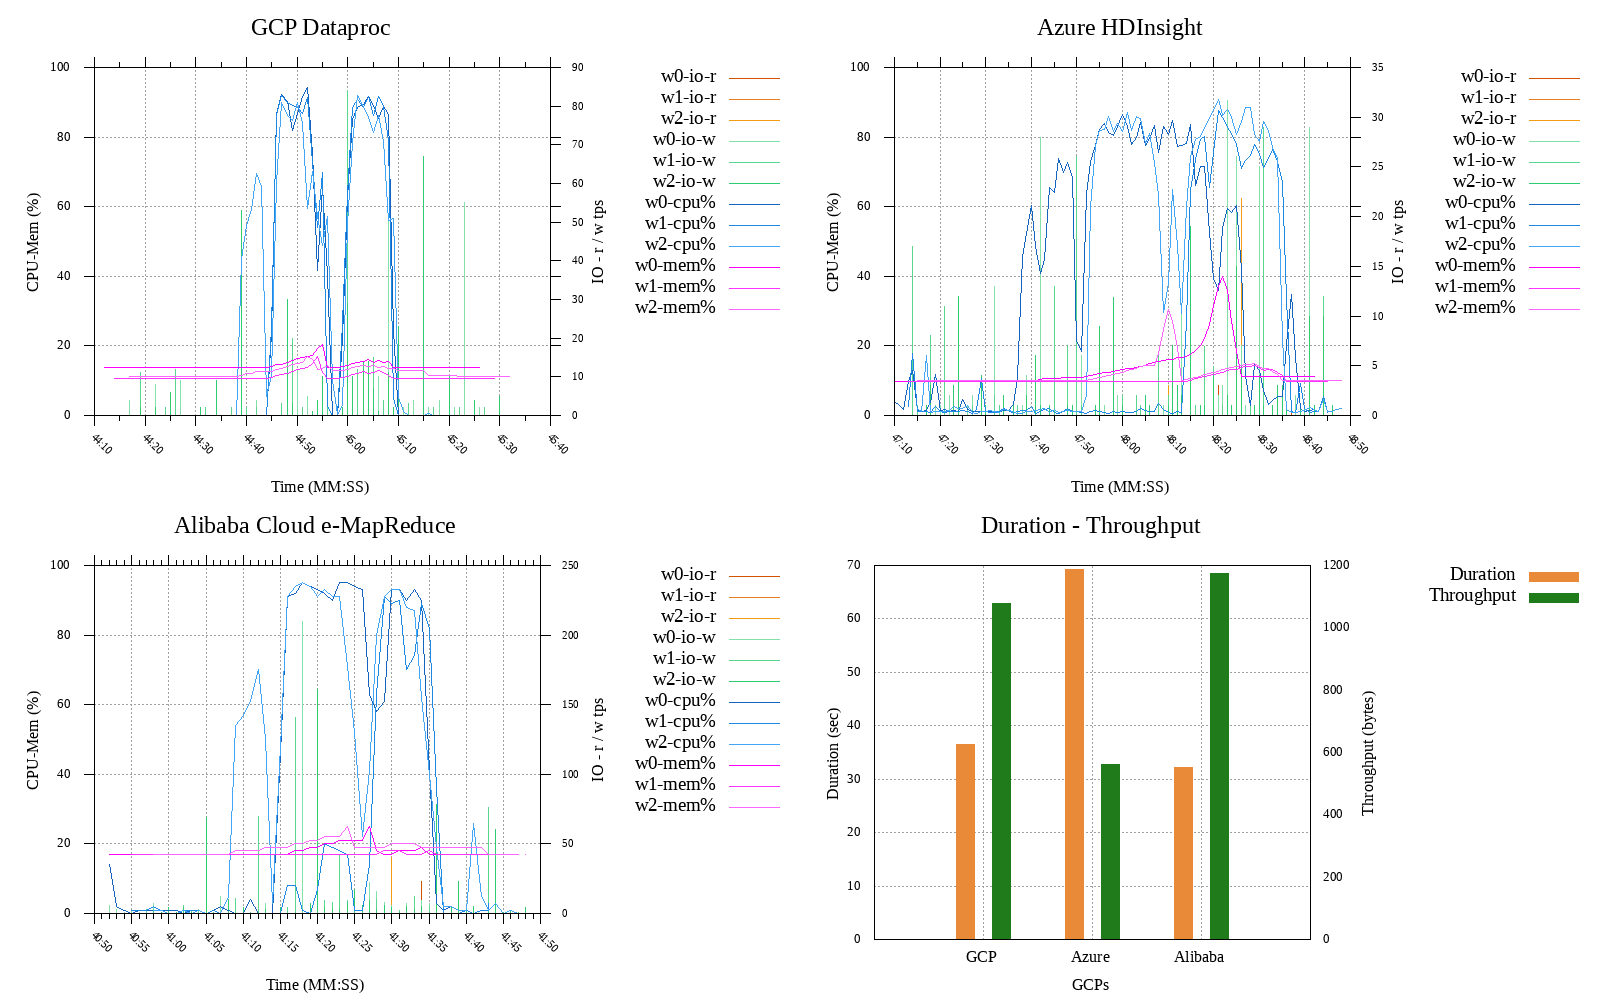
\includegraphics[width=\textwidth]{uc2-srt-t-cmidt}
	\centering
\end{figure}

\begin{figure}[b]
	\caption{UC2 - Sort (Small; 3.2 MB)}
	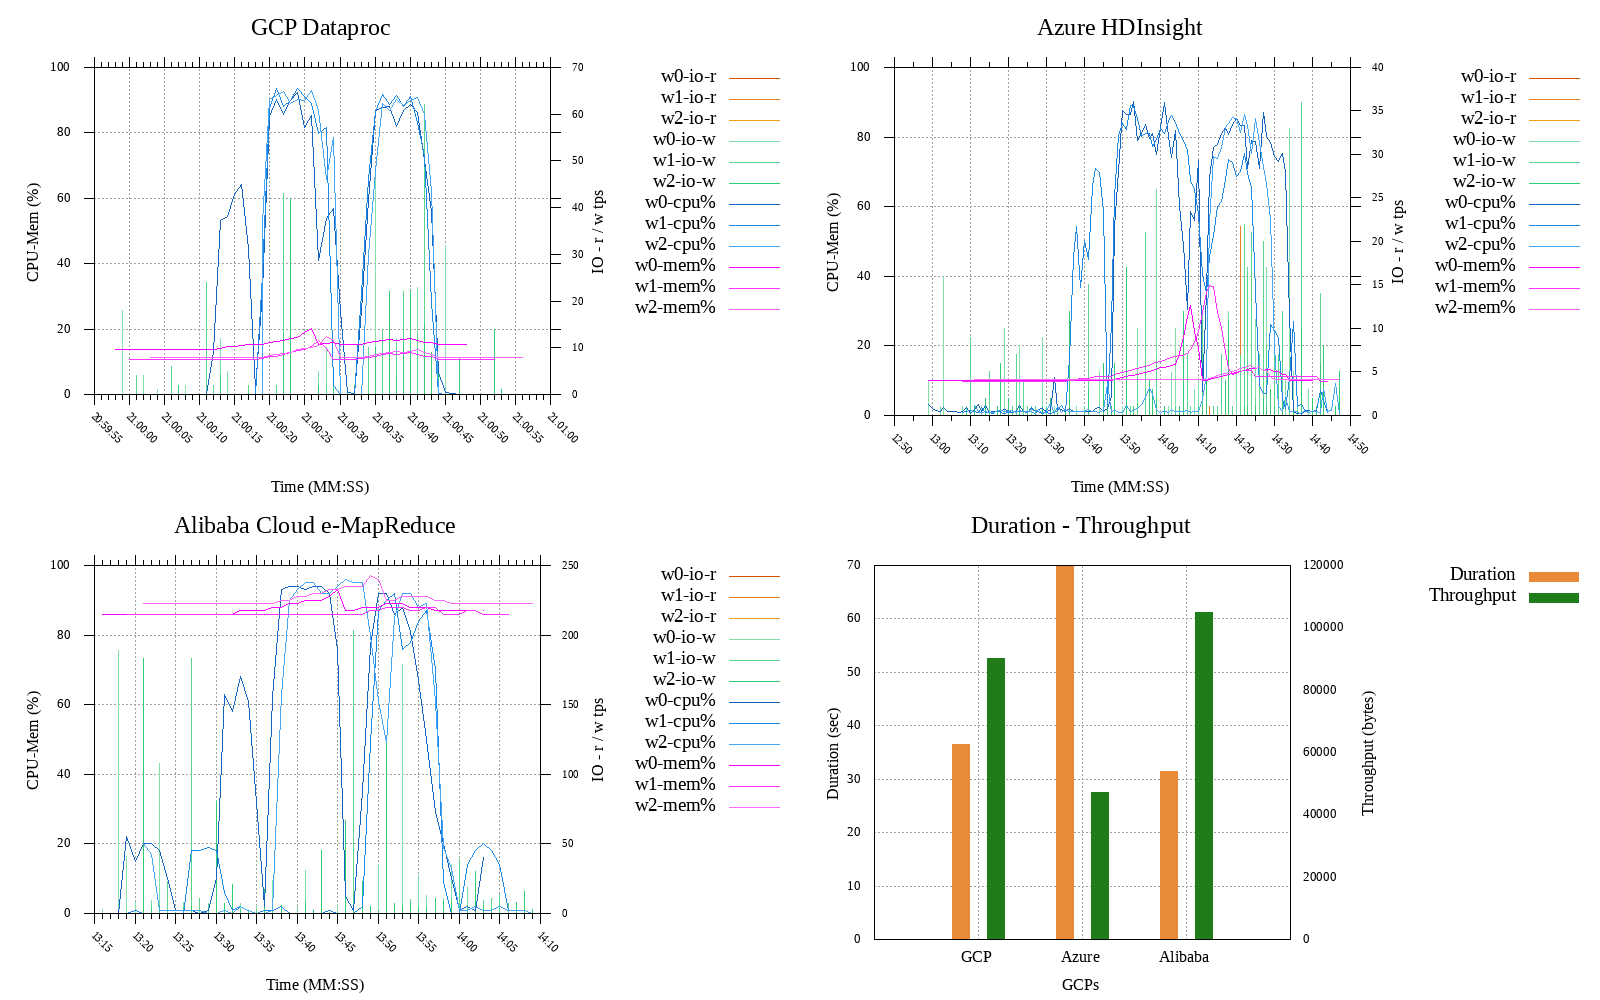
\includegraphics[width=\textwidth]{uc2-srt-s-cmidt}
	\centering
\end{figure}

\begin{figure}[b]
	\caption{UC2 - Sort (Large; 320 MB)}
	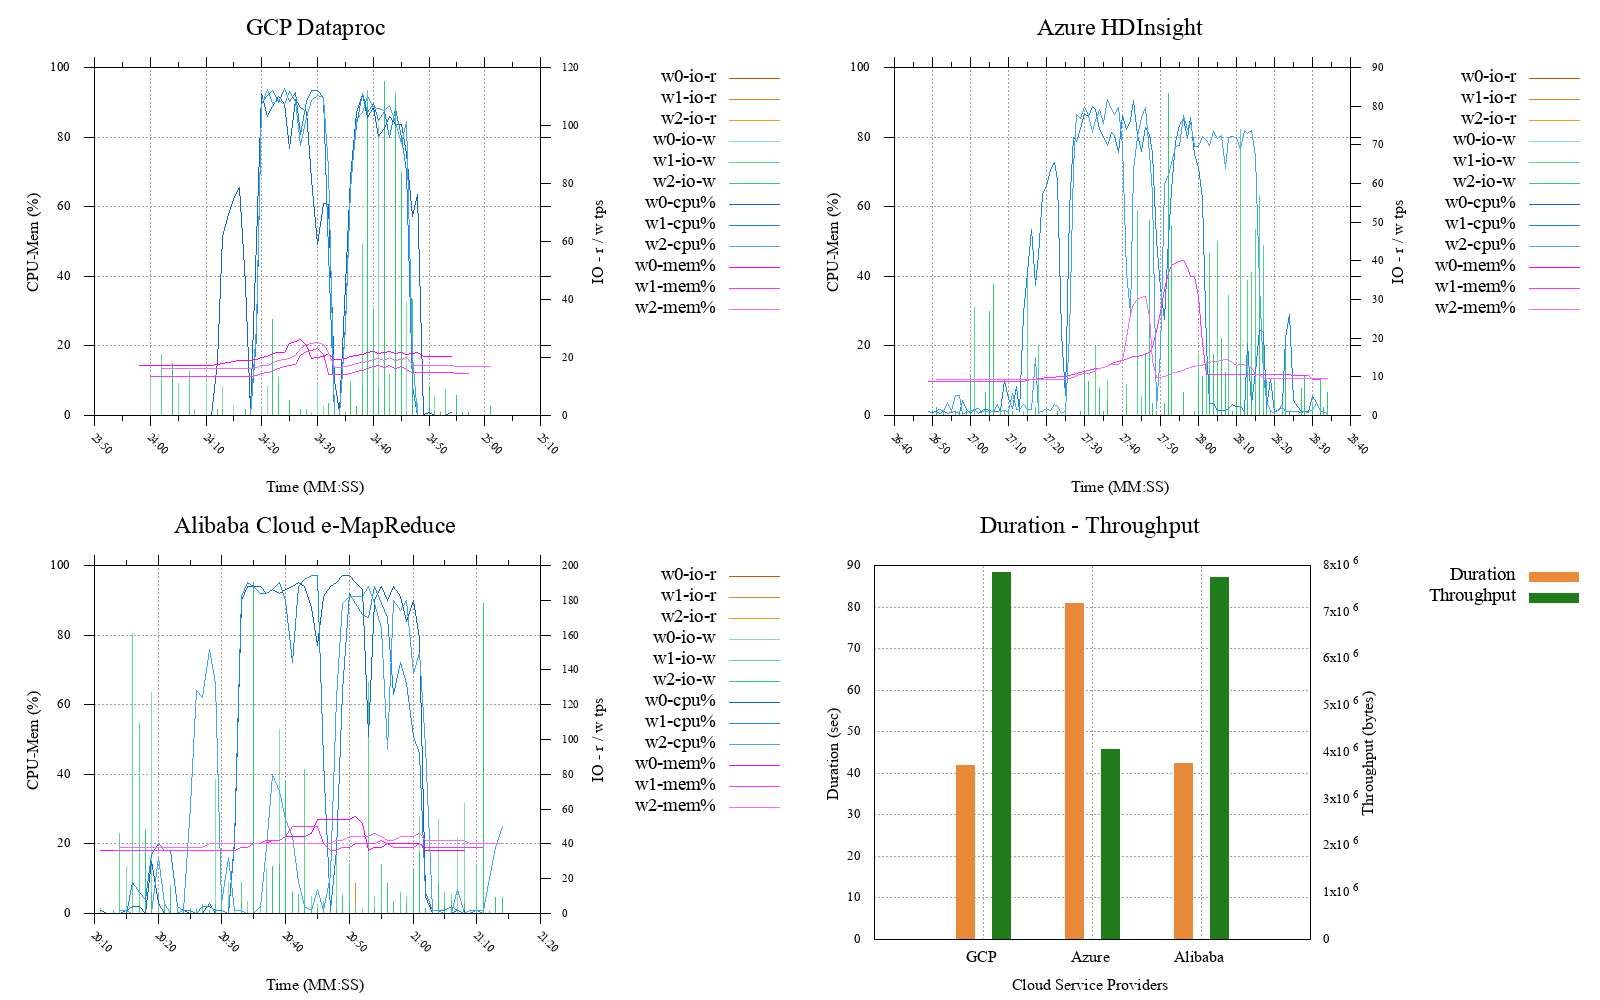
\includegraphics[width=\textwidth]{uc2-srt-l-cmidt}
	\centering
\end{figure}

\begin{figure}[b]
	\caption{UC2 - Sort (Huge; 3.2 GB)}
	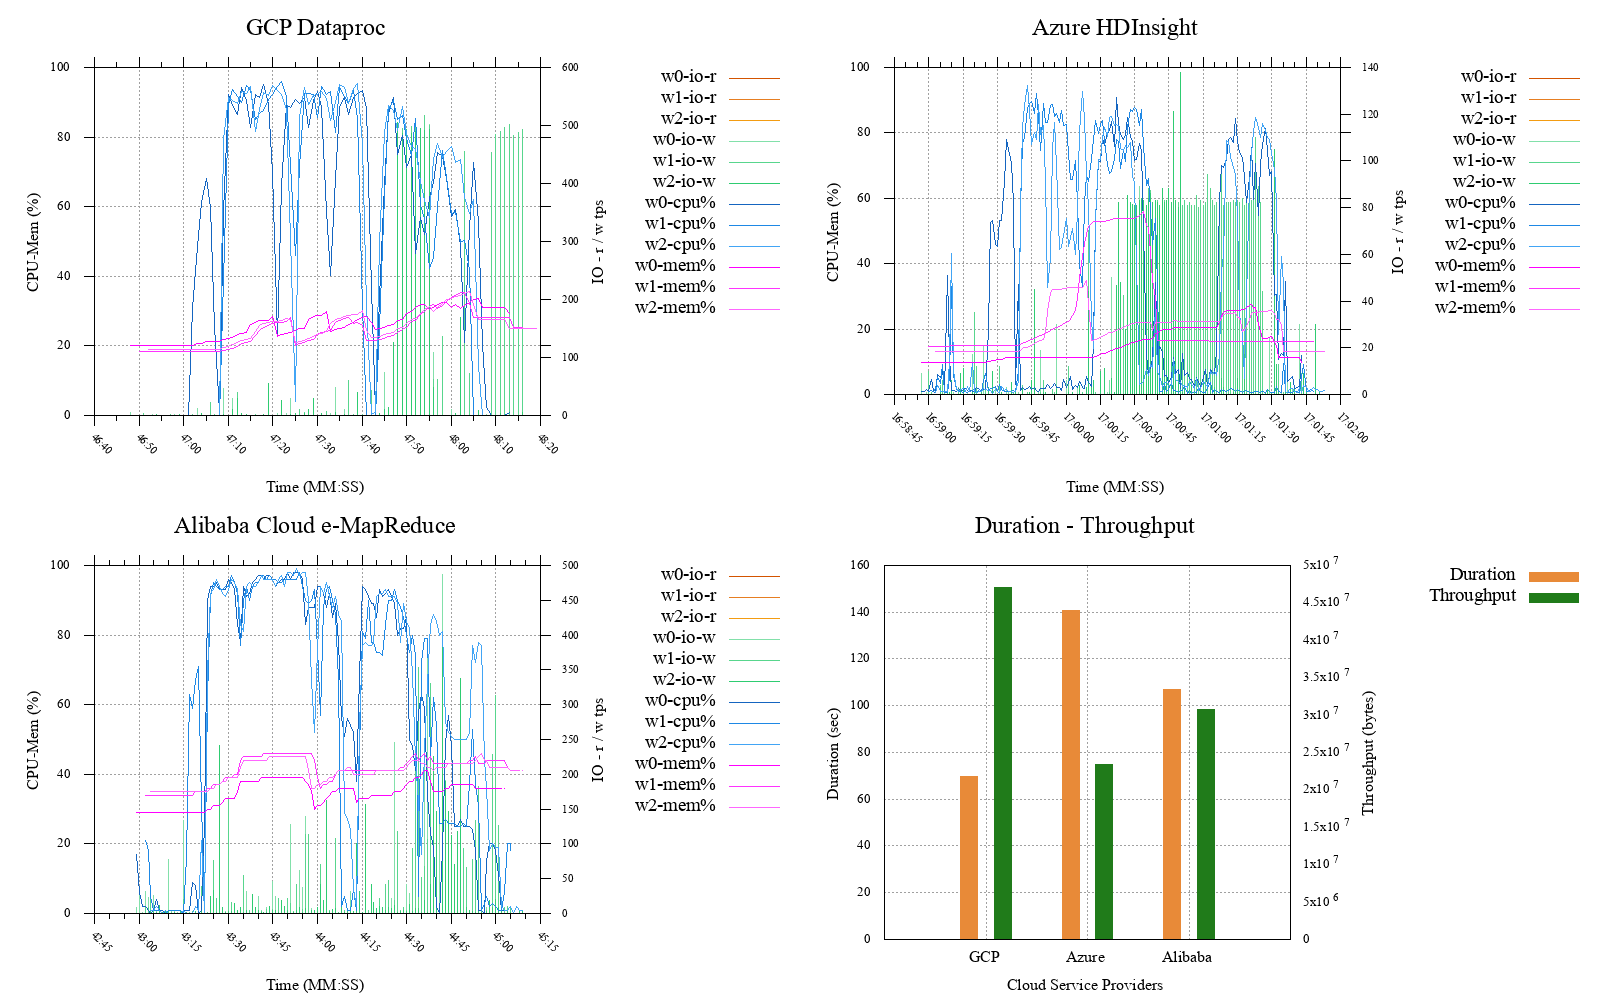
\includegraphics[width=\textwidth]{uc2-srt-h-cmidt}
	\centering
\end{figure}

\begin{figure}[b]
	\caption{UC2 - Sort (Gigantic; 32 GB)}
	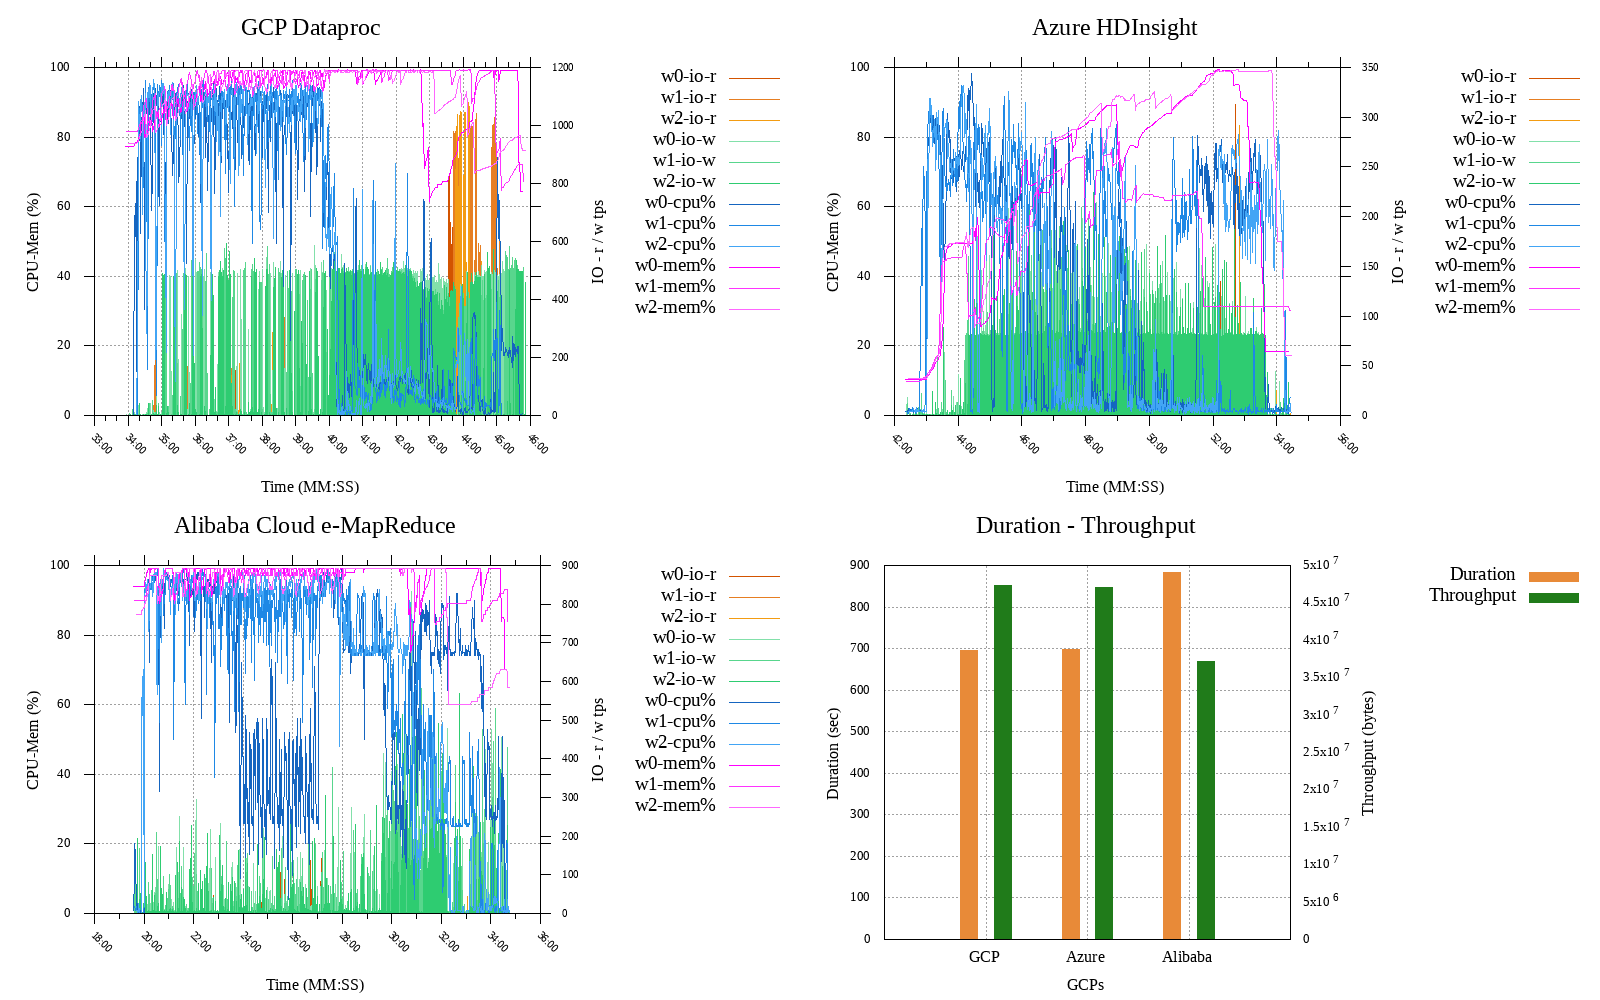
\includegraphics[width=\textwidth]{uc2-srt-g-cmidt}
	\centering
\end{figure}

Wordcount results in scale

\begin{figure}[b]
	\caption{UC2 - Wordcount (Tiny; 32 KB)}
	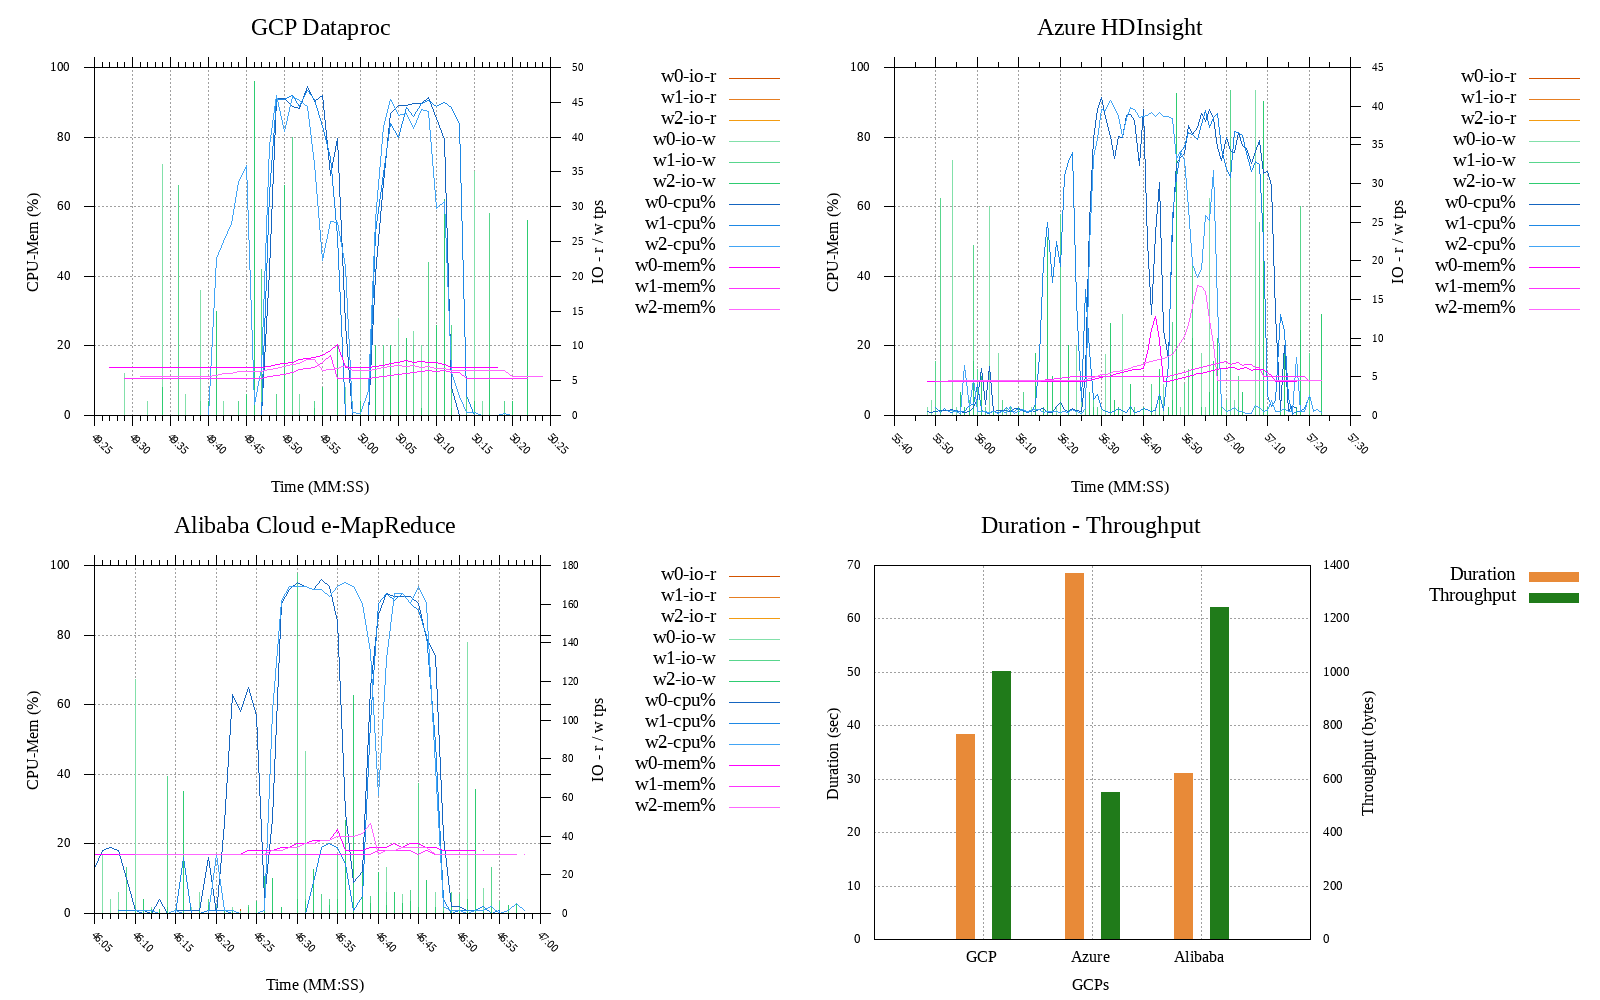
\includegraphics[width=\textwidth]{uc2-wrdcnt-t-cmidt}
	\centering
\end{figure}

\begin{figure}[b]
	\caption{UC2 - Wordcount (Small; 320 MB)}
	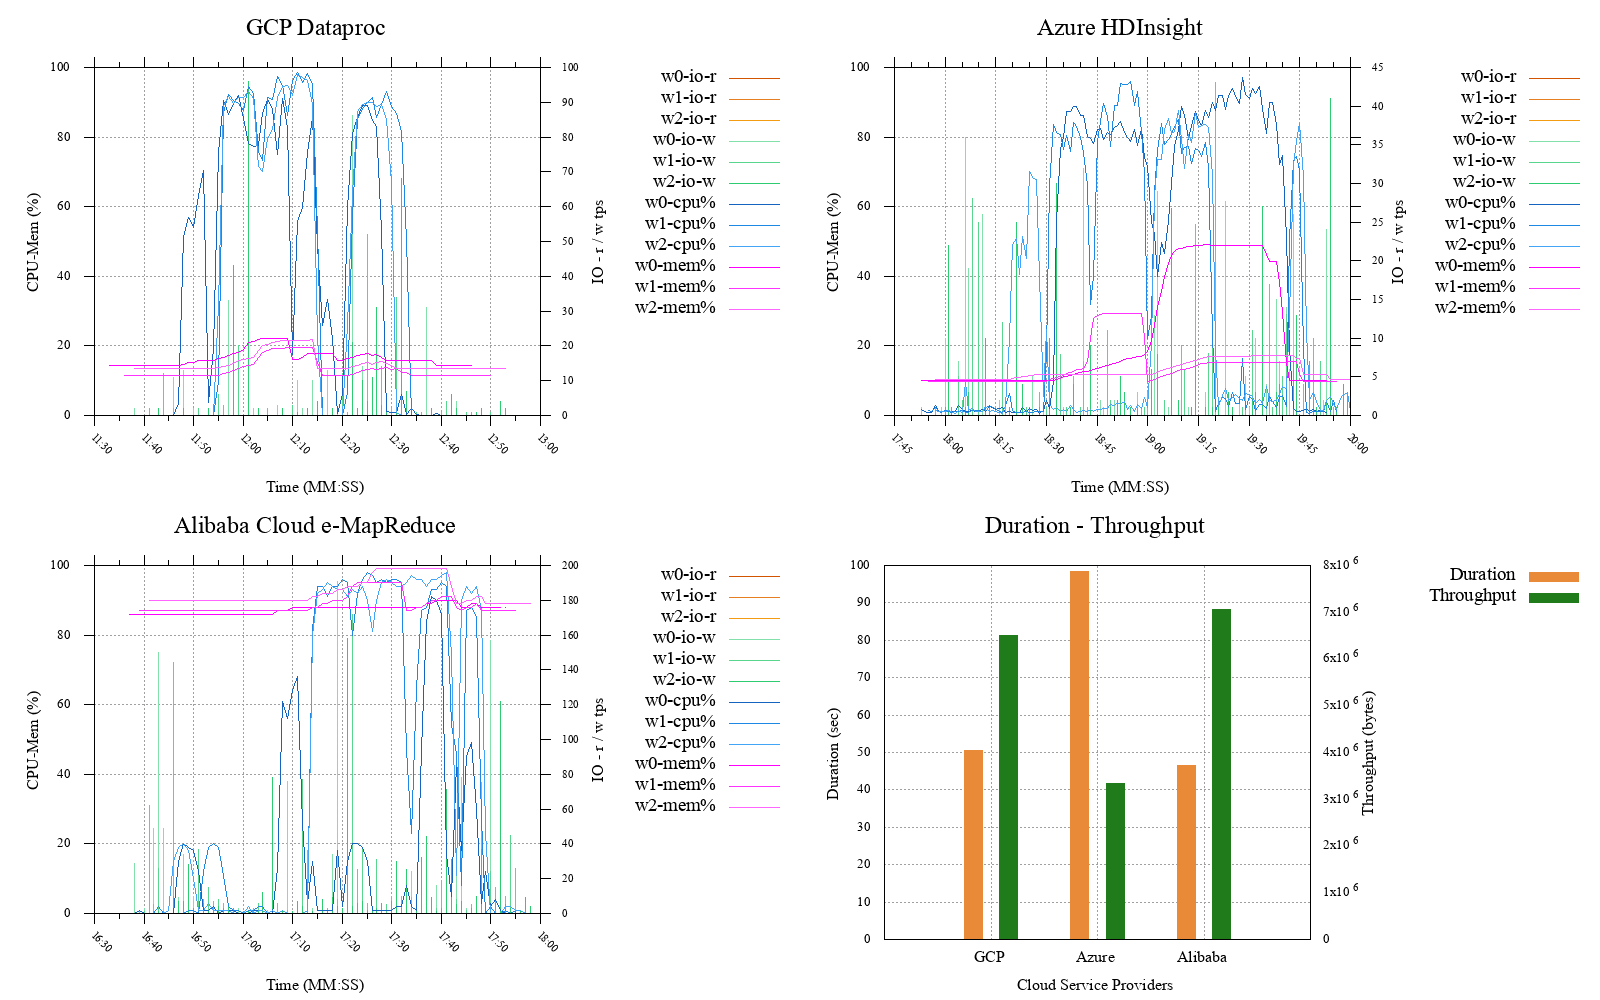
\includegraphics[width=\textwidth]{uc2-wrdcnt-s-cmidt}
	\centering
\end{figure}

\begin{figure}[b]
	\caption{UC2 - Wordcount (Large; 3.2 GB)}
	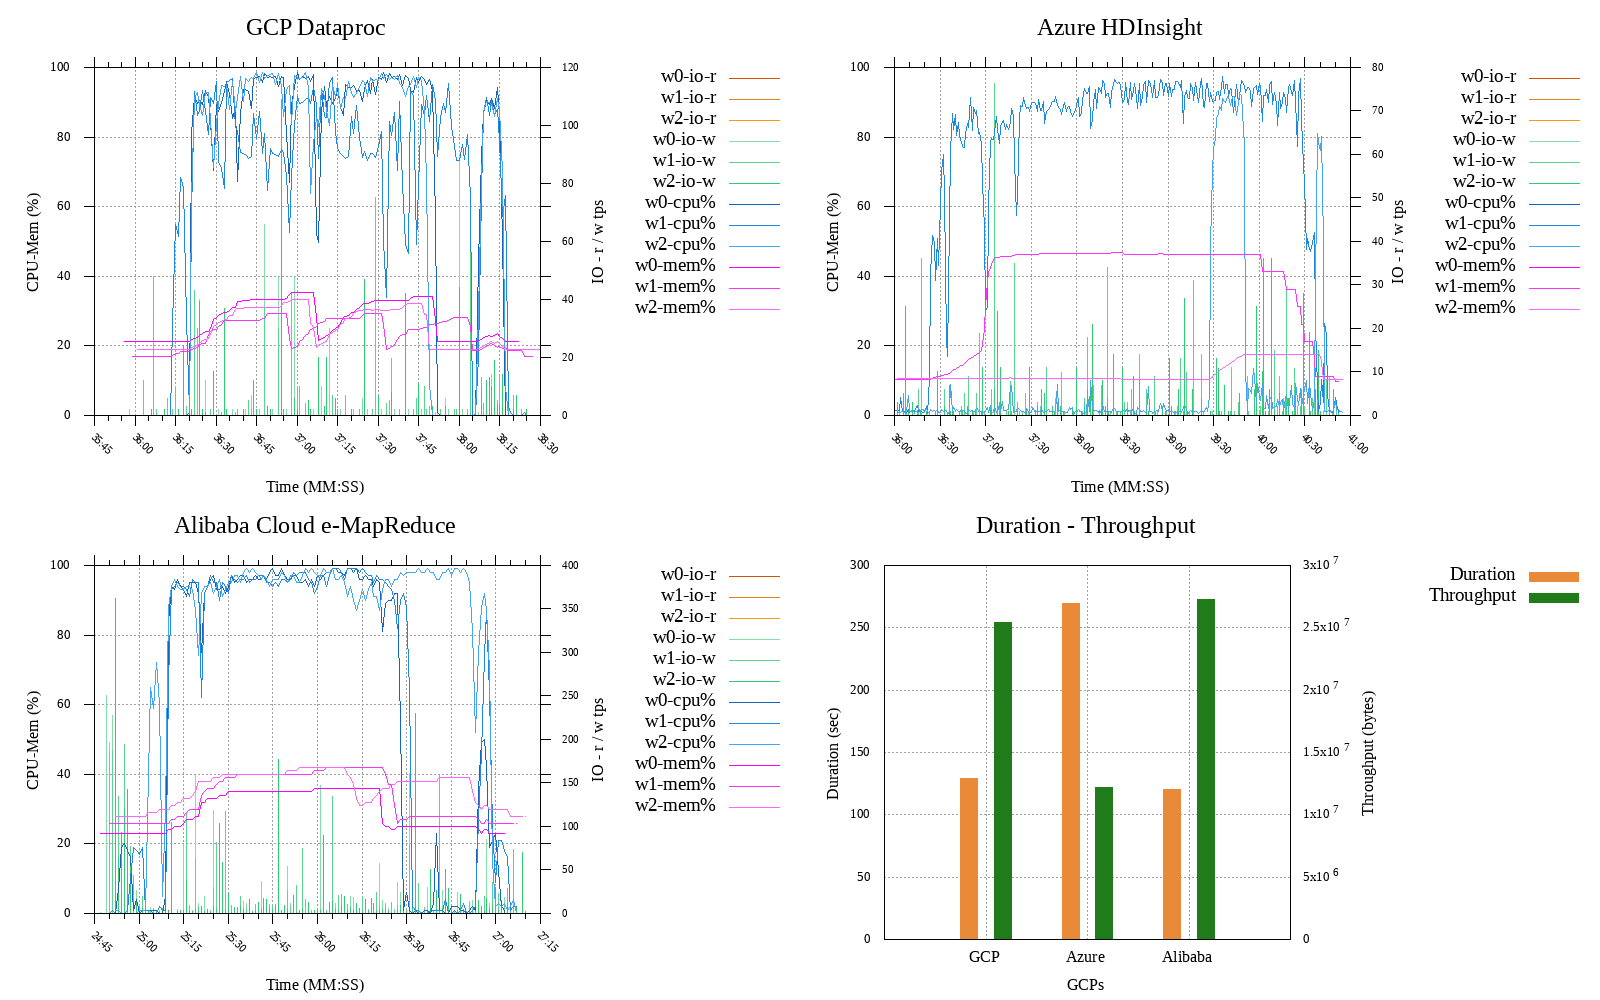
\includegraphics[width=\textwidth]{uc2-wrdcnt-l-cmidt}
	\centering
\end{figure}

\begin{figure}[b]
	\caption{UC2 - Wordcount (Huge; 32 GB)}
	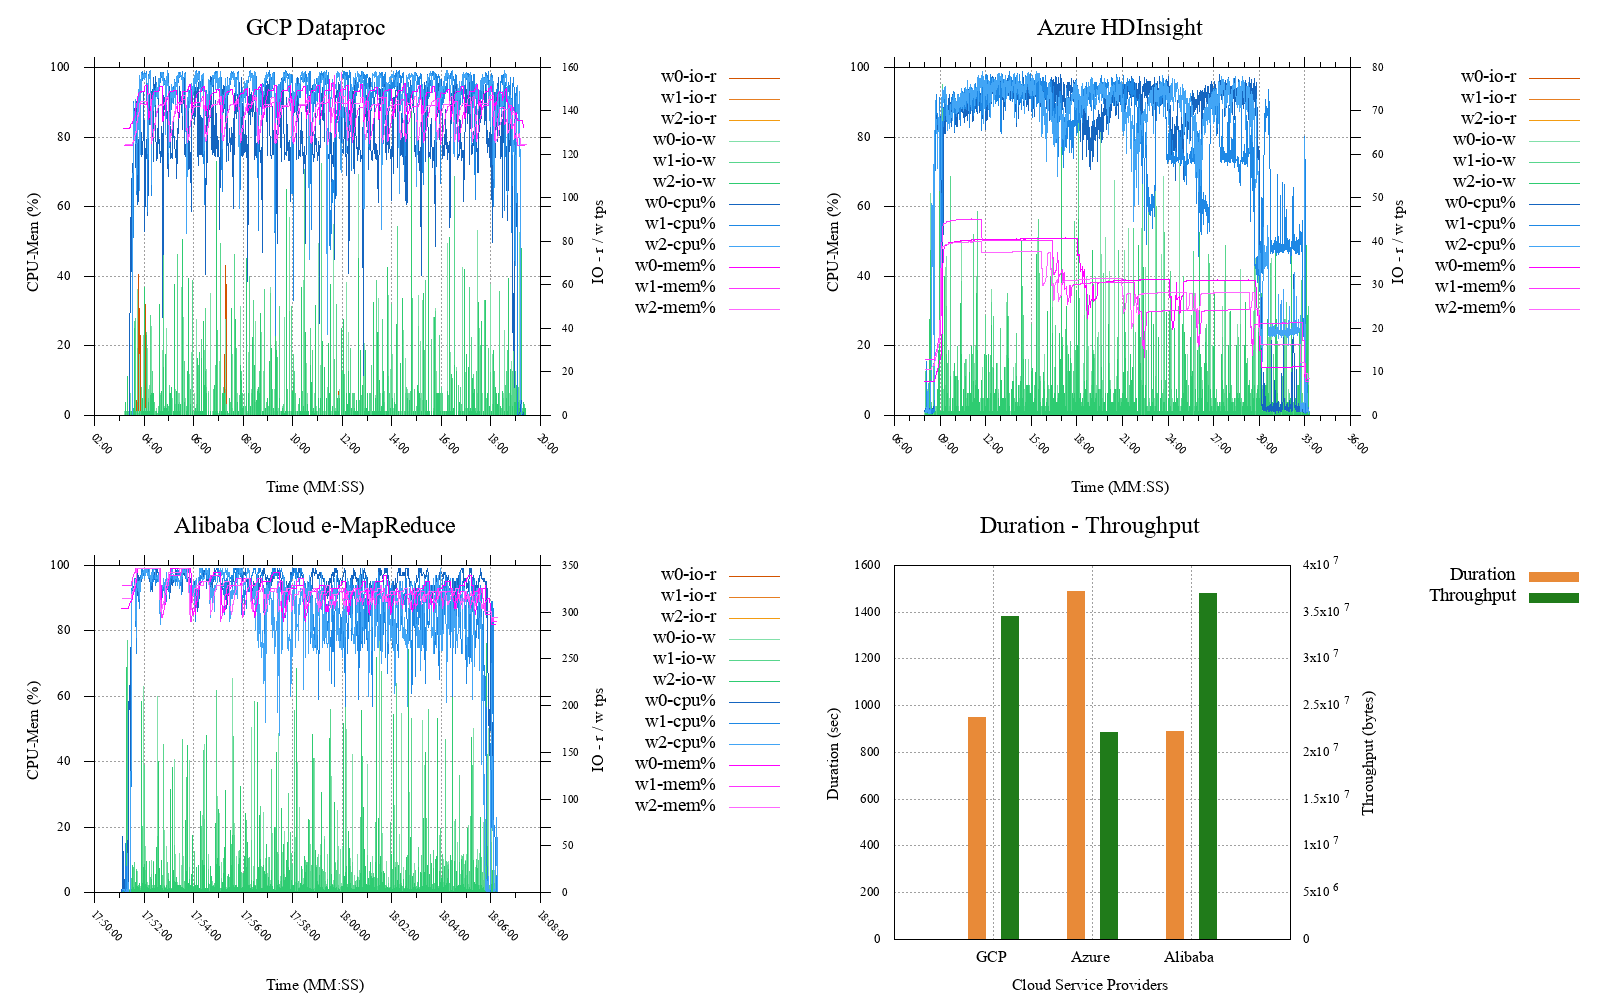
\includegraphics[width=\textwidth]{uc2-wrdcnt-h-cmidt}
	\centering
\end{figure}

\begin{figure}[b]
	\caption{UC2 - Wordcount (Gigantic; 320 GB)}
	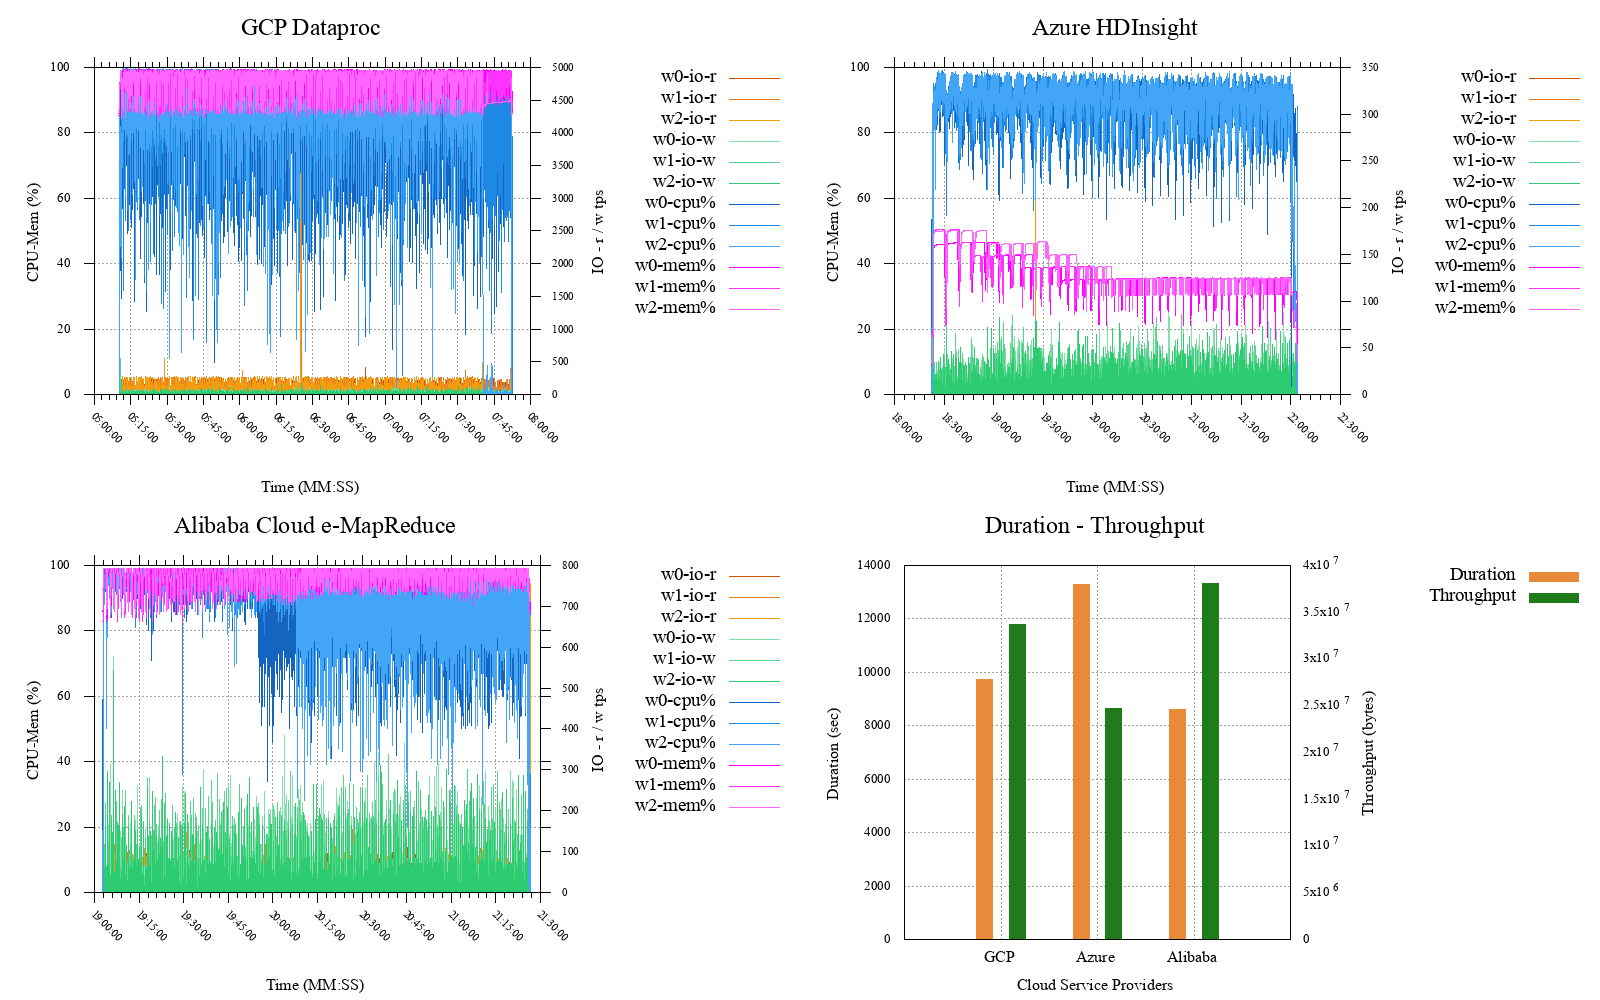
\includegraphics[width=\textwidth]{uc2-wrdcnt-g-cmidt}
	\centering
\end{figure}



\section{Discussion}

\section{Front matter}

The author names and affiliations could be formatted in two ways:
\begin{enumerate}[(1)]
\item Group the authors per affiliation.
\item Use footnotes to indicate the affiliations.
\end{enumerate}
See the front matter of this document for examples. You are recommended to conform your choice to the journal you are submitting to.

\section{Bibliography styles}

There are various bibliography styles available. You can select the style of your choice in the preamble of this document. These styles are Elsevier styles based on standard styles like Harvard and Vancouver. Please use Bib\TeX\ to generate your bibliography and include DOIs whenever available.

Here are two sample references: \cite{Feynman1963118,Dirac1953888}.

\bibliography{mybibfile}

\end{document}